\documentclass[aspectratio=169]{beamer} % Ho mantenuto aspectratio=169 per il formato panoramico

% --- PACCHETTI BASE ---
\usepackage[T1]{fontenc}
\usepackage[utf8]{inputenc}
\usepackage{graphicx}
\usepackage[english]{babel} % Impostato su english poiché le tue slide sono in inglese
\usepackage{booktabs}
\usepackage{amsmath}
\usepackage{xcolor}
\usepackage{tikz}
\usetikzlibrary{patterns,decorations.pathreplacing,positioning,arrows.meta}

% --- IMPOSTAZIONI TEMA E COLORI (Dal tuo template) ---
\usetheme{Ilmenau}
\usecolortheme{beaver}

% Definizione del colore rosso personalizzato
\definecolor{Darkcandyapplered}{rgb}{0.64, 0.0, 0.0}

% Rimozione dei simboli di navigazione in basso a destra
\setbeamertemplate{navigation symbols}{}

% Personalizzazione dei colori per i blocchi e i titoli delle slide
\setbeamercolor{block title}{bg=Darkcandyapplered, fg=white}
\setbeamercolor{frame title}{fg=Darkcandyapplered}

% Personalizzazione del piè di pagina (footline)
\setbeamertemplate{footline}{\leavevmode%
	\begin{beamercolorbox}[wd=.50\paperwidth,left,ht=2.5ex,dp=1.5ex,rightskip=4pt
		plus 1pt, leftskip=4pt]{subsection in head/foot}
		 \insertshortinstitute
	\end{beamercolorbox}%
	\begin{beamercolorbox}[wd=.50\paperwidth,,ht=2.5ex,dp=1.5ex,leftskip=4pt plus 1pt,rightskip=4pt plus 1pt]{section in head/foot}
		\usebeamercolor[fg]{section in foot/head}\insertshortdate\hfill\insertframenumber/\inserttotalframenumber
	\end{beamercolorbox}%
}

% --- INFORMAZIONI DELLA TESI ---
\title[Multi-Objective PrPA]{Balancing KPIs through Multi-Objective\\Prescriptive Process Analytics}
\subtitle{Master's Thesis Presentation}
\author{Daniele Gelmini}
\institute[UniPD - Daniele Gelmini]{Mathematic's Department “Tullio Levi-Civita”\\Università degli Studi di Padova}
\date{August 2026}

\begin{document}

\frame{\titlepage}
\section{Introduction}
\begin{frame}[plain,c]
    \centering
    \color{Darkcandyapplered}
    \Huge\textbf{Introduction}
\end{frame}
\begin{frame}{Background \& Motivation}
    \begin{itemize}
        \item \textbf{Prescriptive Process Analytics (PrPA):} Aims to recommend the next optimal activity and resource to improve Key Performance Indicators (KPIs).
        \item \textbf{Baseline Limitation:} The previous approach aggregates KPIs into a single utility function using an \textit{a priori} $\lambda$ trade-off weight.
        \item \textbf{Drawback:} Training a single predictive model restricts flexibility. Adjusting the strategic trade-off requires completely retraining the model.
    \end{itemize}
\end{frame}

\begin{frame}{Proposed Framework Enhancements}
    \begin{block}{From \textit{A Priori} to \textit{A Posteriori}}
        Instead of selecting $\lambda$ beforehand, the new approach generates multiple optimal solutions, allowing decision-makers to select the desired trade-off \textit{a posteriori} without retraining.
    \end{block}
    \vspace{0.3cm}
    \textbf{Key Modifications:}
    \begin{itemize}
        \item \textbf{Independent Models:} Train a distinct model for each individual KPI.
        \item \textbf{Pareto Front Generation:} Evaluate and store all optimal non-dominated solutions during the recommendation phase.
        \item \textbf{Predictive uncertainty as a confidence filter:} a candidate enters the
          Pareto front only if it is likely enough to beat the ``no recommendation''
          baseline on both KPIs; both models are calibrated post-hoc.
    \end{itemize}
\end{frame}

\begin{frame}{Model Architectures Comparison}
    \begin{columns}
        \begin{column}{0.5\textwidth}
            \centering
            \textbf{Original Architecture} \\
            \vspace{0.2cm}
            \includegraphics[width=\linewidth]{diagramma_old.png} \\
            \vspace{0.1cm}
            \footnotesize{(Single utility model, \textit{a priori} $\lambda$)}
        \end{column}
        \begin{column}{0.5\textwidth}
            \centering
            \textbf{Proposed Architecture} \\
            \vspace{0.2cm}
            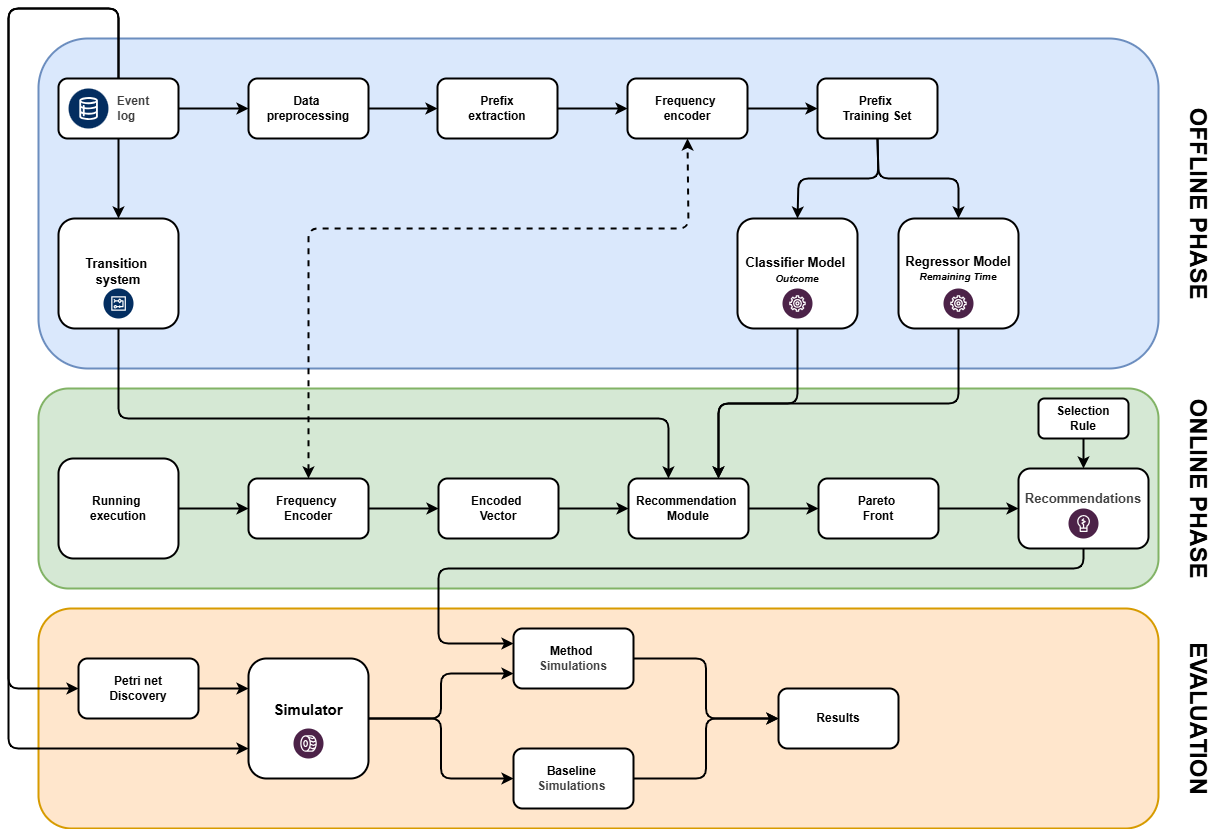
\includegraphics[width=\linewidth]{diagramma.drawio.png} \\
            \vspace{0.1cm}
            \footnotesize{(Multi-model, Pareto Front generation)}
        \end{column}
    \end{columns}
\end{frame}

\section{Offline Phase}

\begin{frame}[plain,c]
    \centering
    \color{Darkcandyapplered}
    \Huge\textbf{Offline Phase}
\end{frame}

% =====================================================================
% START-TIME ESTIMATION
% =====================================================================
\begin{frame}{Start-Time Estimation: the Problem}
  \small
  \begin{itemize}
    \item Each event has a \texttt{start:timestamp} and a \texttt{time:timestamp}
      (completion); the model \textbf{features} and the \textbf{simulator}
      (execution vs.\ waiting times) both rely on the start.
    \item In \textbf{BPI12}, \textbf{bpi17-before}, \textbf{bpi17-after} the recorded
      start is \alert{fake}: a copy of the completion of the previous event of the
      same case.
    \item Consequences:
      \begin{itemize}
        \item every activity starts the instant its predecessor ends
          $\Rightarrow$ \alert{waiting time always 0};
        \item the whole gap (queueing, off-hours, customer delays) is counted as
          \alert{processing time}, and the simulator learns it as such;
        \item \texttt{time\_from\_previous\_event(start)} just repeats the duration of
          the previous event.
      \end{itemize}
    \item \textbf{BAC} records real starts $\Rightarrow$ left untouched.
  \end{itemize}
\end{frame}

\begin{frame}{Start-Time Estimation: the Technique}
  \footnotesize
  Chapela-Campa \& Dumas, \textit{Repairing Activity Start Times to Improve Business
  Process Simulation} (2022), \texttt{pix-framework} implementation:
  \[
    \widehat{\text{start}}(e) = \max\bigl(\text{enabled}(e),\ \text{available}(e)\bigr)
  \]
  \vspace{-0.5cm}
  \begin{itemize}
    \item \textbf{enabled}$(e)$: end of the \emph{causal} predecessor of $e$ in its case
      (latest earlier event not concurrent with $e$, per a concurrency oracle).
    \item \textbf{available}$(e)$: end of the latest earlier event of the \emph{same
      resource} (one activity at a time).
  \end{itemize}
  \vspace{0.1cm}
  \centering
  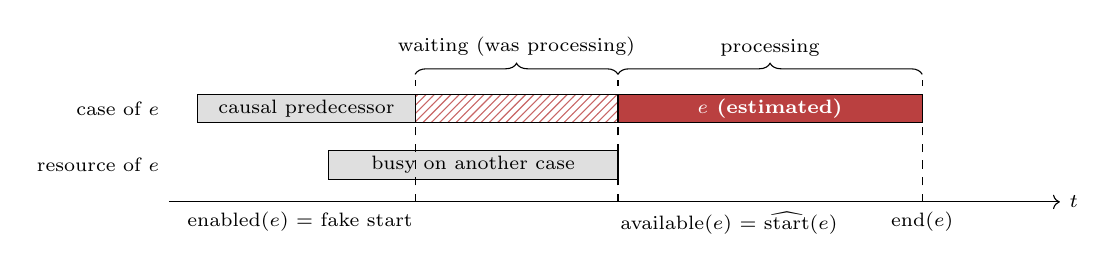
\begin{tikzpicture}[x=0.92cm,y=0.72cm,font=\scriptsize]
    \node[anchor=east] at (0,2) {case of $e$};
    \node[anchor=east] at (0,1) {resource of $e$};
    \draw[->] (0,0.35) -- (12.3,0.35) node[anchor=west] {$t$};
    % predecessor in the case
    \draw[fill=gray!25] (0.4,1.75) rectangle (3.4,2.25);
    \node at (1.9,2) {causal predecessor};
    % resource busy on another case
    \draw[fill=gray!25] (2.2,0.75) rectangle (6.2,1.25);
    \node at (4.2,1) {busy on another case};
    % fake part of e (waiting) and estimated part of e
    \draw[pattern=north east lines, pattern color=Darkcandyapplered!60] (3.4,1.75) rectangle (6.2,2.25);
    \draw[fill=Darkcandyapplered!75] (6.2,1.75) rectangle (10.4,2.25);
    \node[white] at (8.3,2) {\textbf{$e$ (estimated)}};
    % markers
    \draw[dashed] (3.4,0.35) -- (3.4,2.5);
    \draw[dashed] (6.2,0.35) -- (6.2,2.5);
    \draw[dashed] (10.4,0.35) -- (10.4,2.5);
    \node[below left] at (3.5,0.35) {enabled$(e)$ = fake start};
    \node[below right] at (6.1,0.35) {available$(e)$ = $\widehat{\text{start}}(e)$};
    \node[below] at (10.4,0.35) {end$(e)$};
    % braces
    \draw[decorate,decoration={brace,amplitude=4pt}] (3.4,2.6) -- (6.2,2.6)
      node[midway,above=3pt] {waiting (was processing)};
    \draw[decorate,decoration={brace,amplitude=4pt}] (6.2,2.6) -- (10.4,2.6)
      node[midway,above=3pt] {processing};
  \end{tikzpicture}
\end{frame}

\begin{frame}{Start-Time Estimation: Configuration}
  \small
  \begin{itemize}
    \item \textbf{Concurrency oracle:} Heuristics-Miner dependency measures
      (thresholds $0.9$), to find each event's causal predecessor.
    \item \textbf{Domain knowledge} (loan-application processes):
      \begin{itemize}
        \item \texttt{A\_} (application) and \texttt{O\_} (offer) events are state
          changes recorded by the system $\rightarrow$ \alert{instantaneous}
          (start $=$ end); only \texttt{W\_} work items get a duration;
        \item system accounts (\texttt{112} in BPI12, \texttt{User\_1} in BPI17)
          $\rightarrow$ instantaneous;
        \item unknown resource \texttt{0} (BPI12) $\rightarrow$ start $=$ enabled
          time (no availability constraint).
      \end{itemize}
    \item Starts that cannot be estimated are filled with the activity's median
      duration.
  \end{itemize}
\end{frame}

\begin{frame}{Start-Time Estimation: Effect on the Logs}


  \begin{itemize}
    \item Most of the former ``processing time'' is actually \alert{waiting}: the
      simulator can now attribute it to resource availability and calendars.
    \item The repaired log replaces the original as input of the whole pipeline.
  \end{itemize}
\end{frame}

% =====================================================================
% ENCODING & TRAINING INPUT
% =====================================================================
\begin{frame}{Frequency Encoder: From Traces to Feature Vectors}
    \begin{itemize}
        \item Traces have variable length, but the predictive models need a fixed-size numeric input: this is the role of the \textbf{Frequency Encoder} in the architecture diagram -- it turns a prefix of \emph{any} length into a fixed-size feature vector.
        \item \textbf{Core mechanism -- activity frequency counts:} for every activity in the log, a running counter column \texttt{\# ACTIVITY=<name>} tracks how many times that activity has already occurred in the prefix -- a bag-of-activities-style representation, independent of the prefix length.
        \item \textbf{Engineered temporal features:} time elapsed since trace start, time since the previous event, and the duration of the last completed event.
        \item \textbf{Case/event attributes:} categorical fields (activity, resource, weekday, and case-specific attributes) are one-hot encoded; continuous fields (e.g., requested amount) are standardized.
    \end{itemize}
\end{frame}

\begin{frame}{Training Input: One Row per Prefix}
  \small
  Each event $e_i$ of a training case yields one row: the \alert{state} of the case
  after $e_i$ has completed, plus the step that \alert{actually followed} it.
  \vspace{0.4cm}
  \begin{center}
  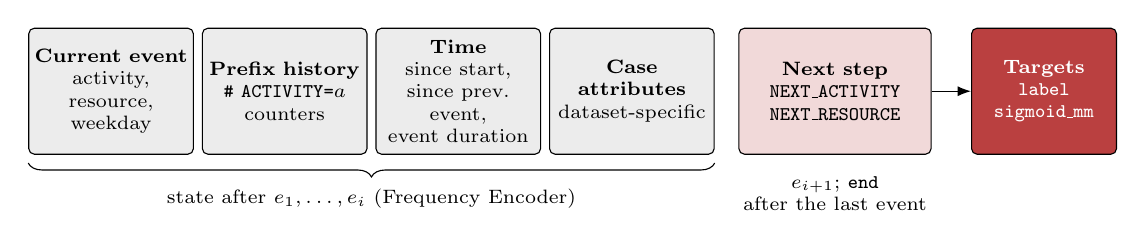
\begin{tikzpicture}[
      box/.style={draw, rounded corners=2pt, align=center, minimum height=1.6cm,
                  text width=1.95cm, font=\scriptsize, inner sep=2pt},
      node distance=0.1cm]
    \node[box, fill=gray!15] (cur) {\textbf{Current event}\\activity, resource,\\weekday};
    \node[box, fill=gray!15, right=of cur] (hist) {\textbf{Prefix history}\\\texttt{\# ACTIVITY=}$a$\\counters};
    \node[box, fill=gray!15, right=of hist] (time) {\textbf{Time}\\since start,\\since prev.\ event,\\event duration};
    \node[box, fill=gray!15, right=of time] (attr) {\textbf{Case}\\\textbf{attributes}\\dataset-specific};
    \node[box, fill=Darkcandyapplered!15, right=0.3cm of attr, text width=2.3cm] (next) {\textbf{Next step}\\\texttt{NEXT\_ACTIVITY}\\\texttt{NEXT\_RESOURCE}};
    \node[box, fill=Darkcandyapplered!75, text=white, right=0.5cm of next, text width=1.7cm] (y) {\textbf{Targets}\\\texttt{label}\\\texttt{sigmoid\_mm}};
    \draw[-{Latex}] (next) -- (y);
    \draw[decorate,decoration={brace,amplitude=5pt,mirror}]
      ([yshift=-3pt]cur.south west) -- ([yshift=-3pt]attr.south east)
      node[midway,below=6pt,font=\scriptsize] {state after $e_1,\dots,e_i$ (Frequency Encoder)};
    \node[below=0.15cm of next, font=\scriptsize, align=center] {$e_{i+1}$; \texttt{end}\\after the last event};
  \end{tikzpicture}
  \end{center}
\end{frame}

\begin{frame}{Training Input: Next Step and Targets}
  \begin{itemize}
    \item \textbf{Why the next step is an input:} at recommendation time
      \texttt{NEXT\_ACTIVITY} / \texttt{NEXT\_RESOURCE} are replaced by each candidate
      \texttt{(activity, resource)} pair, so the models answer
      ``what happens if the case continues \emph{with this step}?''.
    \item \textbf{Targets}:
      \begin{itemize}
        \item \texttt{label}: case outcome (1 $=$ positive, defined per dataset),
          the same for all rows of a case $\rightarrow$ classifier;
        \item \texttt{sigmoid\_mm}: remaining time after $e_i$, z-normalised
          $\rightarrow$ sigmoid $\rightarrow$ min-max to $[0,1]$ $\rightarrow$ regressor.
      \end{itemize}
    \item Case id and timestamps are not model inputs.
    
  \end{itemize}
\end{frame}

\begin{frame}{Training Input: an Example Row (BPI12)}
  \small
  Case \texttt{173721}, 9th event (current training set).
  \begin{center}
  \scriptsize
  \begin{tabular}{lll}
    \toprule
    \textbf{Column} & \textbf{Value} & \textbf{Meaning} \\
    \midrule
    \texttt{concept:name}      & \texttt{W\_Complete\_preaccepted\_appl} & activity just completed \\
    \texttt{org:resource}      & \texttt{10939}  & who executed it \\
    \texttt{weekday}           & Saturday        & day of its start \\
    \texttt{AMOUNT\_REQ}       & 9000            & requested amount (case attr.) \\
    \texttt{\# ACTIVITY=A\_SUBMITTED}, \dots & 1 (8 counters), 0 (15) & activities before $e_i$ \\
    \texttt{time\_from\_start} & 794.8\,s & start($e_i$) - start($e_1$) \\
    \texttt{time\_from\_previous\_event(start)} & 0.03\,s & start($e_i$) - start($e_{i-1}$) \\
    \texttt{event\_duration}   & 1.3\,s & end($e_i$)  - start($e_i$) \\
    \midrule
    \texttt{NEXT\_ACTIVITY} / \texttt{NEXT\_RESOURCE} & \texttt{W\_Call\_after\_offer} / \texttt{10939} & step that followed \\
    \midrule
    \texttt{label}            & 0     & \texttt{O\_ACCEPTED} never occurs \\
    \texttt{remaining\_time} $\rightarrow$ \texttt{sigmoid\_mm} & 9.2 d $\rightarrow$ 0.239 & regression target \\
    \bottomrule
  \end{tabular}
  \end{center}
\end{frame}

\begin{frame}{The ``No Recommendation'' Baseline: What Changed}
  \small
  Reference for a candidate on prefix $e_1,\dots,e_k$: \alert{what if we recommend
  nothing?}
  \vspace{0.1cm}
  \begin{columns}[T]
    \begin{column}{0.49\textwidth}
      \begin{block}{Before}
        \scriptsize
        The prefix \emph{one step shorter} $e_1,\dots,e_{k-1}$, with its real next
        step $e_k$ (a transition already observed).
        \begin{itemize}\scriptsize
          \item \alert{different state} from the candidates: the difference mixes the
            suggestion with the progress of the case (the remaining time still
            includes $e_k$);
          \item not ``nothing'', but a step that already happened;
          \item missing for single-event prefixes.
        \end{itemize}
      \end{block}
    \end{column}
    \begin{column}{0.49\textwidth}
      \begin{block}{Now}
        \scriptsize
        The \emph{same} query instance $e_1,\dots,e_k$ with \texttt{NEXT\_ACTIVITY}
        $=$ \texttt{NEXT\_RESOURCE} $=$ \texttt{\_\_NO\_NEXT\_\_}.
        \begin{itemize}\scriptsize
          \item models trained on a \alert{doubled dataset}: \texttt{\_\_NO\_NEXT\_\_}
            is a value they have learned;
          \item candidate and baseline differ \alert{only in the next step}: a true
            ``suggestion vs.\ nothing'' comparison;
          \item available for every prefix, including single-event ones.
        \end{itemize}
      \end{block}
    \end{column}
  \end{columns}
\end{frame}

\begin{frame}{Training Input: the Doubled Dataset}
  \small
  Every training row is kept \alert{and} copied with the next step blanked out;
  all other features and both targets are unchanged.
  \begin{center}
  \scriptsize
  \begin{tabular}{llllcc}
    \toprule
     & \textbf{State} $e_1,\dots,e_i$ & \texttt{NEXT\_ACTIVITY} & \texttt{NEXT\_RESOURCE} & \texttt{label} & \texttt{sigmoid\_mm} \\
    \midrule
    original & BPI12 case \texttt{173721}, $i=9$ & \texttt{W\_Call\_after\_offer} & \texttt{10939} & 0 & 0.239 \\
    copy     & (identical)                      & \texttt{\_\_NO\_NEXT\_\_} & \texttt{\_\_NO\_NEXT\_\_} & 0 & 0.239 \\
    \bottomrule
  \end{tabular}
  \end{center}
  \footnotesize
  \begin{itemize}
    \item \textbf{Original rows} teach $\mathbb{E}[\,y \mid \text{state},\ \text{next step}\,]$:
      the effect of a specific \texttt{(activity, resource)} $\rightarrow$ scores the
      \emph{candidates}.
    \item \textbf{Copies} teach $\mathbb{E}[\,y \mid \text{state}\,]$: the targets from
      the state alone, averaged over what historically followed similar states
      $\rightarrow$ the \emph{baseline}.
  \end{itemize}
\end{frame}



\begin{frame}{Training Input: BAC}
  \footnotesize
  \textbf{Process:} closure of bank accounts (request, authorisation, pending
  checks, completion). 15 activities, 654 resources.
  \begin{center}
  \begin{tabular}{lp{9.2cm}}
    \toprule
    \textbf{Column} & \textbf{Meaning} \\
    \midrule
    \texttt{CLOSURE\_TYPE} (4 values) & kind of closure: Inheritance, Client Recess, Bank Recess, Porting \\
    \texttt{CLOSURE\_REASON} (9 values) & why the account is closed (e.g.\ ``Client lost'', ``Keep bank account. Same dip'') \\
    \texttt{org:role} (3 values) & role of the executing resource: APPLICANT, DIRECTOR, BACK-OFFICE \\
    15 \texttt{\# ACTIVITY} counters & e.g.\ \texttt{\# ACTIVITY=Authorization Requested} \\
    \midrule
    \texttt{label} $=1$ & the case contains \emph{neither} ``Back-Office Adjustment Requested''
      \emph{nor} ``Network Adjustment Requested'' (no rework) \\
    \bottomrule
  \end{tabular}
  \end{center}
  \begin{itemize}
    \item The two adjustment activities define the outcome $\Rightarrow$
      \alert{forbidden} as recommendations.
    \item Only dataset with real start times; shortest cases (median 7 events).
  \end{itemize}
\end{frame}

\begin{frame}{Training Input: BPI12}
  \footnotesize
  \textbf{Process:} loan applications of a Dutch bank (BPIC 2012). 23 activities,
  61 resources; \texttt{W\_} labels translated to English.
  \begin{center}
  \begin{tabular}{lp{9.2cm}}
    \toprule
    \textbf{Column} & \textbf{Meaning} \\
    \midrule
    \texttt{AMOUNT\_REQ} (continuous) & loan amount requested by the customer \\
    \texttt{A\_} counters & application state changes (e.g.\ \texttt{A\_SUBMITTED}, \texttt{A\_PREACCEPTED}) \\
    \texttt{O\_} counters & offer state changes (e.g.\ \texttt{O\_CREATED}, \texttt{O\_SENT}) \\
    \texttt{W\_} counters & manual work items (e.g.\ \texttt{W\_Call\_after\_offer}, \texttt{W\_Assess\_fraud}) \\
    \midrule
    \texttt{label} $=1$ & an offer is accepted: \texttt{O\_ACCEPTED} occurs in the case \\
    \bottomrule
  \end{tabular}
  \end{center}
  \begin{itemize}
    \item \texttt{O\_ACCEPTED} is \alert{forbidden} as a recommendation.
    \item Most balanced outcome ($48.3\%$ positive), longest cases (median 22 events),
      no categorical case attributes.
  \end{itemize}
\end{frame}

\begin{frame}{Training Input: bpi17-before \& bpi17-after}
  \footnotesize
  \textbf{Process:} loan applications of the same bank (BPIC 2017), two sub-logs with
  their own models. 24 activities, 98 / 107 resources.
  \begin{center}
  \begin{tabular}{lp{8.5cm}}
    \toprule
    \textbf{Column} & \textbf{Meaning} \\
    \midrule
    \texttt{RequestedAmount} (continuous) & loan amount requested \\
    \texttt{LoanGoal} (13 / 14 values) & purpose of the loan (Car, Home improvement, \dots) \\
    \texttt{ApplicationType} (2 values) & New credit / Limit raise \\
    \texttt{EventOrigin} (3 values) & object the event refers to: Application, Offer, Workflow \\
    \texttt{Action} (3 values) & Created, statechange, Deleted \\
    24 \texttt{\# ACTIVITY} counters & \texttt{A\_}, \texttt{O\_}, \texttt{W\_} activities, as in BPI12 \\
    \midrule
    \texttt{label} $=1$ & \texttt{O\_Accepted} occurs in the case \\
    \bottomrule
  \end{tabular}
  \end{center}
  \begin{itemize}
    \item Same columns in both sub-logs (in bpi17-after with the \texttt{case:}
      prefix, e.g.\ \texttt{case:LoanGoal}); \texttt{O\_Accepted} is
      \alert{forbidden} as a recommendation.
  \end{itemize}
\end{frame}

\begin{frame}{Predictive Modeling Strategy}
    \begin{itemize}
        \item The framework leverages independent Machine Learning models tailored to the specific nature of each KPI.
        \item \textbf{Implementation Example:}
        \begin{itemize}
            \item \textbf{CatBoost Regressor:} Used to predict continuous KPIs (e.g., Remaining Execution Time).
            \item \textbf{CatBoost Classifier:} Used to predict discrete or binary KPIs (e.g., Case Outcome probability via \texttt{predict\_proba}).
        \end{itemize}
        \item This decoupling provides higher accuracy and prevents conflicting objectives from diluting a single model's predictive performance.
        \item Both models are trained once, offline, on the encoded prefix training set, and reused for every case and every candidate (activity, resource) pair during the online recommendation phase.
    \end{itemize}
\end{frame}

\begin{frame}{Predictive Uncertainty Quantification}
  \begin{itemize}
    \item A point prediction (a probability, a duration) gives no indication of
      how far it can be trusted.
    \item Two sources of error, estimated separately:
      \begin{itemize}
        \item \alert{Aleatoric} (data) uncertainty: irreducible noise of the
          process; does not shrink with more data.
        \item \alert{Epistemic} (knowledge) uncertainty: the model's ignorance
          on rare or unseen \texttt{(activity, resource)} inputs; shrinks with
          more data, flags out-of-domain candidates.
      \end{itemize}
    \item \textbf{Both} CatBoost models now report this decomposition --- for the
      outcome classifier and the remaining-time regressor.
    \item Online, the per-member predictions are used to estimate the
      \alert{probability that a candidate beats the no-recommendation baseline}
      (confidence filter).
  \end{itemize}

\end{frame}

\begin{frame}{Error decomposition}
    \begin{figure}\centering
        \includegraphics[width=0.78\linewidth]{aleatoric_epistemic.png}
    \end{figure}
\end{frame}

\begin{frame}{Estimating Uncertainty: SGLB \& Virtual Ensembles}
  \begin{itemize}
    \item Both models are trained with \alert{Stochastic Gradient Langevin
      Boosting} (\texttt{posterior\_sampling=True}): Gaussian noise injected in
      the gradient makes the training asymptotically sample the parameter
      posterior $p(\theta \mid \mathcal{D})$.
    \item At inference a \alert{virtual ensemble} is read from the single trained
      model, using truncations of its tree sequence --- an ensemble at the cost
      of one model.
    \item \textbf{Regressor} (\texttt{RMSEWithUncertainty}), law of total
      variance:
      \[
        \underbrace{\sigma_{\text{tot}}^{2}}_{\text{total}} =
        \underbrace{\operatorname{Var}_{m}[\mu_{m}]}_{\text{knowledge}} +
        \underbrace{\tfrac{1}{M}\textstyle\sum_{m}\sigma_{m}^{2}}_{\text{data}}
      \]
    \item \textbf{Classifier}: entropy decomposition: total entropy $=$
      expected member entropy (data) $+$ mutual information (knowledge).
  \end{itemize}
\end{frame}

\begin{frame}{Calibration of the Predictive Models}
  A reported probability or interval is only useful if it matches reality, and
  boosted models tend to be \alert{overconfident}. Each fix is one scalar,
  fitted on a held-out slice, applied to the frozen model.
  \begin{itemize}
    \item \textbf{Classifier $ \rightarrow$ temperature scaling:}
      $p_{\text{cal}} = \sigma\!\left(\sigma^{-1}(p)/T\right)$, $T$ minimising
      log-loss. Monotone $\Rightarrow$ predicted label unchanged, only the
      probability is rescaled. Diagnostic: ECE, before vs after.
    \item \textbf{Regressor $ \rightarrow$ $\sigma$-scaling:} every predicted $\sigma$ is
      multiplied by $s$, minimising the Gaussian NLL; closed form
      $s = \bigl(\tfrac{1}{L}\sum_{j}(y_{j}-\hat y_{j})^{2}/\sigma_{j}^{2}\bigr)^{1/2}$.
      Diagnostics: ENCE and $\pm1\sigma$ / $\pm2\sigma$ coverage
      (target $68\%$ / $95\%$).
  \end{itemize}
\end{frame}

\begin{frame}{Predictive Models: Fit on Train and Test}
  \small
  Classifier: Logloss. Regressor: RMSE and MAE on the normalised
  \texttt{sigmoid\_mm} scale $[0,1]$.
  \begin{center}
  \begin{tabular}{lccccc}
    \hline
     & \multicolumn{2}{c}{Logloss (train / test)} & \multicolumn{2}{c}{RMSE (train / test)} & \multicolumn{1}{c}{Regressor} \\
    \cline{2-3}\cline{4-5}
    Dataset & \multicolumn{2}{c}{Outcome classifier} & \multicolumn{2}{c}{Remaining-time regressor} & \multicolumn{1}{c}{MAE}\\
    \hline
    BAC          & 0.192 & 0.214 & 0.145 & 0.147 & 0.076\\
    BPI12        & 0.501 & 0.530 & 0.198 & 0.242 & 0.183\\
    bpi17-before & 0.473 & 0.488 & 0.201 & 0.248 & 0.189\\
    bpi17-after  & 0.476 & 0.482 & 0.201 & 0.233 & 0.178\\
    \hline
  \end{tabular}
  \end{center}
\end{frame}

\begin{frame}{Predictive Models: Uncertainty \& Calibration}
  \footnotesize
  Test set. Arrows: raw $\rightarrow$ calibrated. ECE / ENCE in \%.
  \begin{center}
  \begin{tabular}{lccccc}
    \hline
    Dataset & ECE & $T$ & ENCE & $s$ & cov.\ $\pm1\sigma$ / $\pm2\sigma$ \\
    \hline
    BAC          & $2.4 \rightarrow$ \textbf{1.9}   & 1.06 & $35.5 \rightarrow 35.4$          & 1.01 & $90 \rightarrow 91$ / $96$\% \\
    BPI12        & $6.5 \rightarrow 6.5$            & 1.00 & $24.2 \rightarrow$ \textbf{15.1} & 1.10 & $60 \rightarrow$ \textbf{65} / $95$\% \\
    bpi17-before & $8.0 \rightarrow 8.4$            & 0.94 & $33.7 \rightarrow$ \textbf{27.7} & 1.07 & $55 \rightarrow$ \textbf{61} / $95$\% \\
    bpi17-after  & $4.3 \rightarrow$ \textbf{4.1}   & 1.06 & $26.6 \rightarrow$ \textbf{23.6} & 1.03 & $59 \rightarrow$ \textbf{62} / $95$\% \\
    \hline
  \end{tabular}
  \end{center}
  \begin{itemize}
    \item \alert{Epistemic} uncertainty is negligible on every dataset
      ($\le 0.1\%$ of the total) --- expected on one-hot tabular inputs; kept
      only as an out-of-domain flag.
    \item Without class weighting the classifiers are already close to calibrated
      ($T = 0.94$--$1.06$): temperature scaling changes ECE little (on bpi17-before
      it rises slightly, $8.0 \rightarrow 8.4\%$, as $T$ is fitted on a held-out slice, not on the test set).
    \item $\sigma$-scaling lowers ENCE (most on BPI12, $24.2 \rightarrow 15.1\%$) and pulls
      $\pm1\sigma$ coverage toward the nominal $68\%$, but on bpi17 it stays below it ($61$--$62\%$).
    \item \textbf{BAC regressor} is the exception: intervals already over-wide
      ($\pm1\sigma$ cov.\ $91\%$), and a single global $s$ cannot fix a
      bin-dependent gap, so ENCE stays $\sim\!35\%$.
  \end{itemize}
\end{frame}

\begin{frame}{Remaining-Time Target: \texttt{sigmoid\_mm} vs.\ Raw Days -- Train \& Test}
  \scriptsize
  Same step-2 training (Optuna 80 trials, \texttt{RMSEWithUncertainty}, $\sigma$-scaling,
  no-recommendation copies); only the regression target changes. No \texttt{idle\_days}.
  Errors in \alert{days} for both targets, computed as the recommender uses the model
  (virtual-ensemble mean; \texttt{sigmoid\_mm} decoded to days, raw days clipped at 0).
  \begin{center}\setlength{\tabcolsep}{5pt}\setlength{\aboverulesep}{0pt}\setlength{\belowrulesep}{1pt}
  \begin{tabular}{llrrrr}
    \toprule
     & & \multicolumn{2}{c}{MAE (d)} & \multicolumn{2}{c}{RMSE (d)} \\
    \cmidrule(lr){3-4}\cmidrule(lr){5-6}
    Dataset (train / test rows) & Target & train & test & train & test \\
    \midrule
    BAC (164257 / 14147)          & sigmoid\_mm & 4.57 & 4.94 & 17.88 & 18.39 \\
                                  & raw days    & 4.96 & 5.60 & 16.21 & 18.16 \\
    \midrule
    BPI12 (91056 / 17119)         & sigmoid\_mm & 6.08 & 8.29 & 9.36  & 12.47 \\
                                  & raw days    & 5.97 & 7.93 & 8.90  & 11.82 \\
    \midrule
    bpi17-before (145832 / 19904) & sigmoid\_mm & 6.75 & 9.62 & 9.73  & 14.34 \\
                                  & raw days    & 6.54 & 9.29 & 9.20  & 13.84 \\
    \midrule
    bpi17-after (166924 / 28394)  & sigmoid\_mm & 6.69 & 8.84 & 9.37  & 13.54 \\
                                  & raw days    & 6.49 & 8.83 & 8.91  & 13.39 \\
    \bottomrule
  \end{tabular}
  \end{center}
  \vspace{-0.2cm}
  \begin{itemize}
    \item Same accuracy: test MAE differs by at most $0.66$ d, test RMSE by at most $0.65$ d.
    \item On the test cases at the split (the recommender's query) the test MAE is
      BAC 11.05 / 10.68, BPI12 6.04 / 6.23, bpi17-before 12.44 / 12.07, bpi17-after 10.09 / 10.19 d
      (\texttt{sigmoid\_mm} / raw days).
  \end{itemize}
  {\scriptsize Train: training rows with their real next step (no-recommendation copies excluded).
  Source: \texttt{2\_training\_results\_realtime.txt}.}
\end{frame}

\begin{frame}{\texttt{sigmoid\_mm} vs.\ Raw Days -- Uncertainty \& Calibration}
  \scriptsize
  Test set. Arrows: raw $\rightarrow$ recalibrated ($\sigma$-scaling). Coverage targets $68\%$ / $95\%$.
  \begin{center}\setlength{\tabcolsep}{5pt}\setlength{\aboverulesep}{0pt}\setlength{\belowrulesep}{1pt}
  \begin{tabular}{llrrrrr}
    \toprule
    Dataset & Target & $s$ & ENCE (\%) & $c_v$ & cov.\ $\pm1\sigma$ (\%) & cov.\ $\pm2\sigma$ (\%) \\
    \midrule
    BAC          & sigmoid\_mm & 1.005 & $35.5 \rightarrow 35.4$ & 0.79 & $90.4 \rightarrow 90.5$ & 96.0 \\
                 & raw days    & 1.071 & $39.3 \rightarrow 38.0$ & 1.03 & $95.9 \rightarrow 96.3$ & 98.5 \\
    \midrule
    BPI12        & sigmoid\_mm & 1.100 & $24.2 \rightarrow 15.1$ & 0.40 & $59.5 \rightarrow 64.6$ & 94.6 \\
                 & raw days    & 1.254 & $39.5 \rightarrow 20.9$ & 0.41 & $70.2 \rightarrow 80.8$ & 94.0 \\
    \midrule
    bpi17-before & sigmoid\_mm & 1.068 & $33.7 \rightarrow 27.7$ & 0.53 & $54.9 \rightarrow 60.5$ & 95.3 \\
                 & raw days    & 1.245 & $55.2 \rightarrow 32.6$ & 0.54 & $62.7 \rightarrow 74.6$ & 91.6 \\
    \midrule
    bpi17-after  & sigmoid\_mm & 1.031 & $26.6 \rightarrow 23.6$ & 0.51 & $58.8 \rightarrow 62.3$ & 94.6 \\
                 & raw days    & 1.175 & $60.1 \rightarrow 42.2$ & 0.49 & $62.7 \rightarrow 73.3$ & 91.0 \\
    \bottomrule
  \end{tabular}
  \end{center}
  \vspace{-0.2cm}
  \begin{itemize}
    \item With raw days the $\pm1\sigma$ coverage rises everywhere: closer to 68\% on bpi17
      (where \texttt{sigmoid\_mm} is overconfident), further above it on BAC and BPI12;
      $\pm2\sigma$ drops to $\sim\!91\%$ on bpi17.
    \item ENCE is worse with raw days on every dataset (larger $s$); $c_v$ is about the same,
      so the uncertainty discriminates between cases equally well.
    \item The time confidence filter uses these $\sigma$: changing target changes which
      candidates pass it.
  \end{itemize}
\end{frame}


\section{Online Phase}

\begin{frame}[plain,c]
    \centering
    \color{Darkcandyapplered}
    \Huge\textbf{Online Phase}
\end{frame}

\begin{frame}{Recommendation Generation}
  \small
  \begin{itemize}
    \item For a running case, the feasibility module returns the valid
      \texttt{(activity, resource)} candidates --- on average
      $\sim\!290\text{--}470$ per prefix, depending on the dataset.
    \item Each candidate is scored by the two models, by placing it in the
      \texttt{NEXT\_ACTIVITY} / \texttt{NEXT\_RESOURCE} columns of the query instance.
    \item \alert{Confidence filter:} a candidate is kept only if it is likely enough
      to beat the \emph{no-recommendation} baseline on both KPIs (next slides).
    \item The survivors are compared on \alert{two objectives}, optimised jointly:
      \begin{itemize}
        \item outcome probability;
        \item $1 -$ predicted remaining time, normalised to $[0,1]$.
      \end{itemize}
    \item The \alert{non-dominated} candidates form the Pareto front.
    \item Exhaustive evaluation: a single vectorised pass over all feasible pairs — exact and, at this scale, fast.
  \end{itemize}
\end{frame}

% =====================================================================
% CONFIDENCE FILTER
% =====================================================================
\begin{frame}{Confidence Filter: Motivation}
  \small
  \begin{itemize}
    \item The Pareto front compares candidates \emph{only with each other}. A
      non-dominated candidate can still be:
      \begin{itemize}
        \item predicted \alert{worse than not intervening} at all;
        \item better only by a margin far \alert{below the model's own uncertainty}.
      \end{itemize}
    \item Earlier version: the predictive standard deviation of the time was a
      \emph{third Pareto objective}. But $\sigma$ alone says how noisy a prediction
      is, not whether the candidate improves on anything, and a noisy candidate
      could still enter the front through the other two axes.
    \item \textbf{New question}, asked for each candidate and each KPI:
      \begin{block}{}
        \centering
        How likely is it that following this candidate is \emph{better} than giving
        no recommendation?
      \end{block}
    \item One number per KPI that combines \alert{effect size} (difference of the
      predictions) and \alert{uncertainty}, readable as a probability
      $\Rightarrow$ a threshold $\gamma$ has a direct meaning.
  \end{itemize}
\end{frame}

\begin{frame}{Confidence Filter: the Baseline}
  \small
  \begin{itemize}
    \item \textbf{Baseline} $B$: the query instance of the case with
      \texttt{NEXT\_ACTIVITY} $=$ \texttt{NEXT\_RESOURCE} $=$ \texttt{\_\_NO\_NEXT\_\_}
      --- the value learned from the doubled training set (offline phase).
    \item It predicts outcome and remaining time from \emph{the same state} as the
      candidates, when the process continues as it historically did.
    \item \textbf{Candidate} $A$: the same query instance with the candidate
      \texttt{(activity, resource)} as next step.
    \item Both are scored by \alert{every member} $m = 1,\dots,M$ of the same
      virtual ensemble ($M \le 50$):
      \begin{itemize}
        \item \textbf{outcome}: calibrated \alert{logit} $a_m, b_m$ --- unbounded,
          so a Gaussian model is sensible (the probability is bounded in $[0,1]$);
          the logit is monotone in the probability, so $P(\text{logit}_A >
          \text{logit}_B) = P(p_A > p_B)$;
        \item \textbf{time}: predicted mean $a_m, b_m$ of \texttt{sigmoid\_mm}, plus each   member's own (aleatoric) variance $\sigma^2_{A,m}$, $\sigma^2_{B,m}$;   the resulting std is multiplied by the $\sigma$-scaling factor $s$ (calibrated).

      \end{itemize}
  \end{itemize}
\end{frame}

\begin{frame}{Confidence Filter: Probability of Beating the Baseline}
  \footnotesize
  $A$ and $B$ modelled as \alert{correlated Gaussians}, with moments estimated from
  the $M$ paired members:
  \[
    \bar d = \bar a - \bar b, \qquad
    s_d^{2} = s_A^{2} + s_B^{2} - 2\, s_{AB}, \qquad
    s_{AB} = \tfrac{1}{M-1}\textstyle\sum_{m}(a_m-\bar a)(b_m-\bar b)
  \]
  \begin{itemize}
    \item \textbf{time}: predicted mean $a_m, b_m$ of \texttt{sigmoid\_mm}, plus each   member's own (aleatoric) variance $\sigma^2_{A,m}$, $\sigma^2_{B,m}$;   the resulting std is multiplied by the $\sigma$-scaling factor $s$ (calibrated).

    \item Posterior predictive of a new difference (normal population, unknown mean
      and variance): $D \sim t_{M-1}\bigl(\bar d,\ s_d^2 (1 + 1/M)\bigr)$, hence
  \end{itemize}
  \[
    P(A > B) = T_{M-1}\!\left(\frac{\bar d}{s_d\sqrt{1 + 1/M}}\right)
  \]
  \vspace{-0.2cm}
  \[
    p_{\text{out}} = P(\text{outcome}_A > \text{outcome}_B), \qquad
    p_{\text{time}} = 1 - P(\text{time}_A > \text{time}_B) \quad \text{(shorter is better)}
  \]
\end{frame}

\begin{frame}{Confidence Filter: Modelling Choices}
  \begin{itemize}
    \item \textbf{Why paired:} member $m$ scores both $A$ and $B$, so their errors are
      positively correlated; assuming independence would overstate $s_d$ and push
      every probability towards $0.5$.
    \item \textbf{Why Student-$t$ and not the normal CDF:} mean and variance are
      \emph{estimated} from only $M$ members; the $t$ distribution with $M-1$ degrees
      of freedom and the $(1+1/M)$ factor account for it, and tend to the plain
      $z$-test as $M \to \infty$.
    \item \textbf{Why the logit for the outcome:} a probability lives in $[0,1]$ and is
      poorly described by a Gaussian; the logit is unbounded and monotone in it.
    \item \textbf{Why only the time uses the aleatoric part:} for the time we compare the remaining times the case may actually take, so each member's own variance $\sigma_m^2$ is part of the prediction. For the outcome we compare the \emph{probabilities} of success: the aleatoric noise of a classifier is the $0/1$ result of the single case, $p_m(1-p_m)$, not uncertainty about $p$ itself, so it does not enter the comparison.

  \end{itemize}
\end{frame}

\begin{frame}{Confidence Filter: the Rule}
  \begin{block}{}
    \centering
    keep candidate $\iff$ $p_{\text{out}} \ge \gamma_{\text{cls}}$ \ \textbf{and} \
    $p_{\text{time}} \ge \gamma_{\text{reg}}$ \qquad (default $\gamma_{\text{cls}} = \gamma_{\text{reg}} = 0.5$)
  \end{block}
  \vspace{0.1cm}
  \centering
  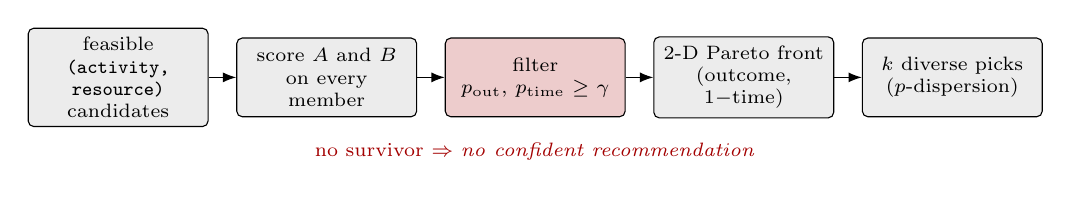
\begin{tikzpicture}[
      stage/.style={draw, rounded corners=2pt, align=center, font=\scriptsize,
                   text width=2.05cm, minimum height=1.0cm, fill=gray!15},
      node distance=0.35cm]
    \node[stage] (c) {feasible\\\texttt{(activity, resource)}\\candidates};
    \node[stage, right=of c] (s) {score $A$ and $B$\\on every member};
    \node[stage, fill=Darkcandyapplered!20, right=of s] (f) {filter\\$p_{\text{out}},\,p_{\text{time}} \ge \gamma$};
    \node[stage, right=of f] (p) {2-D Pareto front\\(outcome, $1-$time)};
    \node[stage, right=of p] (k) {$k$ diverse picks\\($p$-dispersion)};
    \draw[-{Latex}] (c) -- (s); \draw[-{Latex}] (s) -- (f);
    \draw[-{Latex}] (f) -- (p); \draw[-{Latex}] (p) -- (k);
    \node[below=0.2cm of f, font=\scriptsize, align=center, text=Darkcandyapplered]
      {no survivor $\Rightarrow$ \emph{no confident recommendation}};
  \end{tikzpicture}
  \small
  \begin{itemize}
    \item Uncertainty is no longer a Pareto axis: it acts as a \alert{gate} before the
      front, which is built on the two KPIs only.
    \item If nothing survives, the case receives \emph{no} recommendation rather than a
      doubtful one: letting the process continue is itself the safe choice.
    \item $\gamma$ is the minimum required probability of improving on the baseline;
      raising it makes the recommender more conservative.
  \end{itemize}
\end{frame}

% \begin{frame}{Confidence Filter in Practice}
%   \small
%   150 random test prefixes per dataset, all feasible candidates, current models.
%   \begin{center}
%   \begin{tabular}{lcccc}
%     \toprule
%      & \textbf{BAC} & \textbf{BPI12} & \textbf{bpi17-before} & \textbf{bpi17-after} \\
%     \midrule
%     Candidates per prefix           & 394 & 220 & 421 & 515 \\
%     Pass outcome ($\gamma = 0.5$)   & $61.2\%$ & $31.8\%$ & $48.9\%$ & $44.7\%$ \\
%     Pass time ($\gamma = 0.5$)      & $58.3\%$ & $83.4\%$ & $72.4\%$ & $73.5\%$ \\
%     Pass both ($\gamma = 0.5$)      & $32.8\%$ & $25.5\%$ & $31.6\%$ & $29.2\%$ \\
%     Pass both ($\gamma = 0.6$)      & $0.6\%$  & $1.2\%$  & $0.9\%$  & $0.0\%$ \\
%     \bottomrule
%   \end{tabular}
%   \end{center}
%   \footnotesize
%   \begin{itemize}
%     \item At $\gamma = 0.5$ the rule is equivalent to ``predicted mean \alert{no worse}
%       than the baseline'' ($T_{M-1}(z) \ge 0.5 \iff \bar d \ge 0$): it removes
%       about $67\text{--}75\%$ of the candidates.
%     \item \textbf{Time:} the total variance is dominated by the aleatoric part, so
%       $p_{\text{time}}$ stays close to $0.5$ ($74$--$99\%$ of the candidates between
%       $0.4$ and $0.6$, never below $0.05$ or above $0.9$)
%       $\Rightarrow$ $\gamma = 0.6$ already removes almost everything.
%     \item \textbf{Outcome:} only the (negligible) epistemic spread is available, so
%       $p_{\text{out}}$ is mostly $\approx 0$ or $\approx 1$ ($44$--$90\%$ of the
%       candidates below $0.05$ or above $0.95$).
%   \end{itemize}
% \end{frame}

% =====================================================================
% CONFIDENCE FILTER: EFFECT OF GAMMA (3_confidence_filter_sweep.txt)
% =====================================================================
\begin{frame}{Confidence Filter in Practice: BAC}
  \small
  1876 test cases, \alert{all} with at least one feasible candidate from the transition system
  (497.7 per case): every case without a recommendation is removed by the filter. The same $\gamma$ is used for both
  KPIs; $\gamma = 0$: no filter. $\gamma = 0.9$ is omitted: no case has a recommendation, as at 0.8.

  \textbf{Candidates passing the filter, Pareto front, \% of test cases with a recommendation at rank $r$ (at least $r$ recommendations) and with none}
  \begin{center}\setlength{\tabcolsep}{4pt}\setlength{\aboverulesep}{0pt}\setlength{\belowrulesep}{1pt}
  \begin{tabular}{crrrrrrrrrr}
    \toprule
     & \multicolumn{3}{c}{\% candidates passing} & Front & \multicolumn{5}{c}{\% test cases with rank $r$} & No rec. \\
    \cmidrule(lr){2-4}\cmidrule(lr){6-10}
    $\gamma$ & outcome & time & both & size & 1 & 2 & 3 & 4 & 5 & (\% cases) \\
    \midrule
    0 (none) & 100.0 & 100.0 & 100.0 & 1.70 & 100.0 & 44.7 & 18.5 & 4.9 & 1.2 & 0.0 \\
    0.5      & 48.7  & 54.1  & 24.0  & 1.28 & 95.1  & 28.0 & 5.0  & 0.1 & 0.0 & 4.9 \\
    0.6      & 47.5  & 0.3   & 0.3   & 0.39 & 38.3  & 0.6  & 0.0  & 0.0 & 0.0 & 61.7 \\
    0.7      & 47.1  & 0.0   & 0.0   & 0.00 & 0.2   & 0.0  & 0.0  & 0.0 & 0.0 & 99.8 \\
    0.8      & 43.1  & 0.0   & 0.0   & 0.00 & 0.0   & 0.0  & 0.0  & 0.0 & 0.0 & 100.0 \\
    \bottomrule
  \end{tabular}
  \end{center}
\end{frame}

\begin{frame}{Confidence Filter in Practice: BPI12}
  \small
  623 test cases, \alert{all} with at least one feasible candidate from the transition system
  (218.5 per case): every case without a recommendation is removed by the filter. The same $\gamma$ is used for both
  KPIs; $\gamma = 0$: no filter. $\gamma = 0.9$ is omitted: no case has a recommendation, as at 0.8.

  \textbf{Candidates passing the filter, Pareto front, \% of test cases with a recommendation at rank $r$ (at least $r$ recommendations) and with none}
  \begin{center}\setlength{\tabcolsep}{4pt}\setlength{\aboverulesep}{0pt}\setlength{\belowrulesep}{1pt}
  \begin{tabular}{crrrrrrrrrr}
    \toprule
     & \multicolumn{3}{c}{\% candidates passing} & Front & \multicolumn{5}{c}{\% test cases with rank $r$} & No rec. \\
    \cmidrule(lr){2-4}\cmidrule(lr){6-10}
    $\gamma$ & outcome & time & both & size & 1 & 2 & 3 & 4 & 5 & (\% cases) \\
    \midrule
    0 (none) & 100.0 & 100.0 & 100.0 & 2.95 & 100.0 & 99.8 & 64.4 & 17.5 & 12.8 & 0.0 \\
    0.5      & 30.8  & 82.6  & 23.9  & 1.93 & 99.4  & 93.3 & 0.3  & 0.0  & 0.0 & 0.6 \\
    0.6      & 16.4  & 2.3   & 2.3   & 0.45 & 24.7  & 20.4 & 0.0  & 0.0  & 0.0 & 75.3 \\
    0.7      & 16.1  & 0.0   & 0.0   & 0.00 & 0.0   & 0.0  & 0.0  & 0.0  & 0.0 & 100.0 \\
    0.8      & 15.4  & 0.0   & 0.0   & 0.00 & 0.0   & 0.0  & 0.0  & 0.0  & 0.0 & 100.0 \\
    \bottomrule
  \end{tabular}
  \end{center}
\end{frame}

\begin{frame}{Confidence Filter in Practice: bpi17-before}
  \small
  1218 test cases, \alert{all} with at least one feasible candidate from the transition system
  (424.1 per case): every case without a recommendation is removed by the filter. The same $\gamma$ is used for both
  KPIs; $\gamma = 0$: no filter. $\gamma = 0.9$ is omitted: no case has a recommendation, as at 0.8.

  \textbf{Candidates passing the filter, Pareto front, \% of test cases with a recommendation at rank $r$ (at least $r$ recommendations) and with none}
  \begin{center}\setlength{\tabcolsep}{4pt}\setlength{\aboverulesep}{0pt}\setlength{\belowrulesep}{1pt}
  \begin{tabular}{crrrrrrrrrr}
    \toprule
     & \multicolumn{3}{c}{\% candidates passing} & Front & \multicolumn{5}{c}{\% test cases with rank $r$} & No rec. \\
    \cmidrule(lr){2-4}\cmidrule(lr){6-10}
    $\gamma$ & outcome & time & both & size & 1 & 2 & 3 & 4 & 5 & (\% cases) \\
    \midrule
    0 (none) & 100.0 & 100.0 & 100.0 & 5.85 & 100.0 & 100.0 & 96.6 & 87.6 & 78.8 & 0.0 \\
    0.5      & 60.0  & 70.3  & 39.3  & 2.61 & 99.6  & 96.4  & 61.2 & 2.7  & 0.5 & 0.4 \\
    0.6      & 28.3  & 23.3  & 0.6   & 0.68 & 53.7  & 12.1  & 2.4  & 0.0  & 0.0 & 46.3 \\
    0.7      & 28.0  & 12.0  & 0.0   & 0.00 & 0.0   & 0.0   & 0.0  & 0.0  & 0.0 & 100.0 \\
    0.8      & 28.0  & 3.2   & 0.0   & 0.00 & 0.0   & 0.0   & 0.0  & 0.0  & 0.0 & 100.0 \\
    \bottomrule
  \end{tabular}
  \end{center}
\end{frame}

\begin{frame}{Confidence Filter in Practice: bpi17-after}
  \small
  1840 test cases, \alert{4 with no feasible candidate}: the transition system knows no next
  activity for their prefix, so they get no recommendation for any $\gamma$ (they are the 0.2\%
  of ``No rec.'' at $\gamma = 0$); 502.4 candidates per case. The same
  $\gamma$ is used for both KPIs; $\gamma = 0$: no filter. $\gamma = 0.9$ is omitted: no case has a
  recommendation, as at 0.8.

  \textbf{Candidates passing the filter, Pareto front, \% of test cases with a recommendation at rank $r$ (at least $r$ recommendations) and with none}
  \begin{center}\setlength{\tabcolsep}{4pt}\setlength{\aboverulesep}{0pt}\setlength{\belowrulesep}{1pt}
  \begin{tabular}{crrrrrrrrrr}
    \toprule
     & \multicolumn{3}{c}{\% candidates passing} & Front & \multicolumn{5}{c}{\% test cases with rank $r$} & No rec. \\
    \cmidrule(lr){2-4}\cmidrule(lr){6-10}
    $\gamma$ & outcome & time & both & size & 1 & 2 & 3 & 4 & 5 & (\% cases) \\
    \midrule
    0 (none) & 100.0 & 100.0 & 100.0 & 4.88 & 99.8 & 98.0 & 86.4 & 75.7 & 56.4 & 0.2 \\
    0.5      & 59.2  & 73.7  & 42.2  & 1.81 & 99.8 & 70.5 & 8.8  & 1.6  & 0.0 & 0.2 \\
    0.6      & 37.1  & 23.1  & 0.0   & 0.01 & 0.8  & 0.1  & 0.0  & 0.0  & 0.0 & 99.2 \\
    0.7      & 37.0  & 18.7  & 0.0   & 0.00 & 0.0  & 0.0  & 0.0  & 0.0  & 0.0 & 100.0 \\
    0.8      & 35.8  & 9.2   & 0.0   & 0.00 & 0.0  & 0.0  & 0.0  & 0.0  & 0.0 & 100.0 \\
    \bottomrule
  \end{tabular}
  \end{center}
\end{frame}

\begin{frame}{Confidence Filter: Effect of $\gamma$}
  \footnotesize
  \begin{itemize}
    \item \textbf{$\gamma = 0.5$} keeps 24--42\% of the candidates, yet almost every case
      still gets a recommendation (no recommendation: 0.2\% bpi17-after -- 4.9\% BAC).
    \item \textbf{$\gamma = 0.6$} is already too strict: the cases left without a
      recommendation jump to 46\% (bpi17-before), 62\% (BAC), 75\% (BPI12), 99\% (bpi17-after);
      from $\gamma = 0.7$ practically none has one (0.2\% on BAC, 0 elsewhere).
    \item \textbf{The time condition is the bottleneck.} On BAC and BPI12 almost no
      candidate passes it at 0.6 (0.3\%, 2.3\%): the time probabilities sit close to 0.5,
      as the aleatoric noise dominates the difference between candidate and baseline.
      On bpi17 23\% pass on time and 28--37\% on outcome, but almost none on \emph{both}
      (0.6\% and 0.0\%, against 6.6\% and 8.6\% if independent): the candidates
      better on one KPI are rarely better on the other.
    \item \textbf{Fronts are small:} 1.3--2.6 points per case at $\gamma = 0.5$ (1.7--5.9
      without filter), so with $k = 5$ ranks 4--5 are almost always empty; $k = 3$ would
      cover nearly every case.
    \item \textbf{No candidate at all} from the transition system: only 4 cases (bpi17-after);
      every other case without a recommendation is due to the filter.
  \end{itemize}
  {\scriptsize Source: \texttt{3\_confidence\_filter\_sweep.txt}.}
\end{frame}

\begin{frame}{Why Exhaustive Search, Not a Genetic Algorithm}
  A heuristic multi-objective search (genetic / NSGA-II) was implemented and
  compared, then dropped.
  \begin{itemize}
    \item \textbf{Small search space:} on average $\sim\!290\text{--}470$ feasible
      \texttt{(activity, resource)} pairs per prefix. Exhaustive search scores
      each pair \alert{once} and returns the \alert{exact} front.
    \item \textbf{Genetic search pays a warm-up cost:} the front (and its
      hypervolume) only stabilises after several generations, and each
      generation evaluates a whole population through both models --- so
      $\mathrm{pop\_size} \times n_{\text{gen}}$ model calls quickly exceed the
      single exhaustive pass, for a result that is still approximate.

  \end{itemize}

\end{frame}

\begin{frame}{Why Exhaustive Search, Not a Genetic Algorithm}
    \begin{itemize}
        \item \textbf{Measured (per case, EXHAUSTIVE vs NSGA-II):}
    \end{itemize}
    \begin{center}
      \begin{tabular}{lcc}
        \hline
        Case study & Exhaustive & NSGA-II \\
        \hline
        BAC          & $0.31$\,s & $0.55$\,s \\
        BPI12        & $0.16$\,s & $0.98$\,s \\
        bpi17-before & $0.08$\,s & $0.41$\,s \\
        bpi17-after  & $0.09$\,s & $0.42$\,s \\
        \hline
      \end{tabular}
    \end{center}
    \begin{block}{}
        At this scale exhaustive search wins on both quality (exact front) and time.
        A genetic search would only pay off with thousands of candidates
        (e.g.\ hundreds of eligible resources per activity).
    \end{block}
\end{frame}


\begin{frame}{Exploring the Pareto Front \& Time Normalization}
    \begin{itemize}
        \item \textbf{Time Transformation Pipeline:} To harmonize scales and enable multi-objective optimization, raw remaining time undergoes:
        \begin{enumerate}
            \item \textbf{Z-normalization:} Standardizes skewed temporal distributions.
            \item \textbf{Sigmoid Transformation:} Smooths extreme outliers.
            \item \textbf{Min-Max Scaling:} Maps values into the $[0, 1]$ interval.
        \end{enumerate}
        \item \textbf{Inversion ($1 - \text{Time}$):} Converts time minimization into maximization, placing the ideal theoretical point at $(1,1)$ for intuitive visual trade-off analysis.
        \item Predictive uncertainty does not add an axis: it has already been used by
          the confidence filter, so the front lives in $[0,1]^2$.
    \end{itemize}
\end{frame}

\begin{frame}{Selection Rule: Max-Min Dispersion (\textit{p}-Dispersion)}
    \begin{itemize}
        \item Once the Pareto front is computed for a case, the framework selects $k$ representative (activity, resource) candidates to be evaluated in simulation, instead of the whole front.
        \item \textbf{Goal:} spread the $k$ selected points as evenly as possible across the front, rather than clustering them in one region of the objective space.
        \item \textbf{Formulation:} the \textit{max-min dispersion} (\textit{p}-dispersion) problem -- select the subset of $k$ points that maximizes the minimum pairwise distance among the selected points, computed in the min-max normalised (outcome, $1-$time) objective space.
        \item \textbf{Exact solution:} solved to optimality as a MILP (\texttt{spopt.locate.PDispersion}), built from the pairwise Euclidean distance matrix of the front and solved with the CBC solver.
        \item If the front has $k$ points or fewer, all of them are kept.
    \end{itemize}
\end{frame}

\begin{frame}{Experimental Results: Pareto Fronts (BAC)}
    \begin{figure}
        \centering
        \includegraphics[width=0.5\linewidth]{pareto_front_images/pareto_BAC_20191010593_exhaustive.jpg}
    \end{figure}
\end{frame}

\begin{frame}{Experimental Results: Pareto Fronts (BPI12)}
    \begin{figure}
        \centering
        \includegraphics[width=0.5\linewidth]{pareto_front_images/pareto_BPI12_195082_exhaustive.jpg}
    \end{figure}
\end{frame}

\begin{frame}{Experimental Results: Pareto Fronts (bpi17-before)}
    \begin{figure}
        \centering
        \includegraphics[width=0.5\linewidth]{pareto_front_images/pareto_bpi17_before_Application_1290192129_exhaustive.jpg}
    \end{figure}
\end{frame}

\begin{frame}{Experimental Results: Pareto Fronts (bpi17-after)}
    \begin{figure}
        \centering
        \includegraphics[width=0.5\linewidth]{pareto_front_images/pareto_bpi17_after_Application_429482627_exhaustive.jpg}
    \end{figure}
\end{frame}

\begin{frame}{Pareto Front Cardinality}
    \begin{itemize}
        \item Not every case yields an equally rich Pareto front: the number of non-dominated (activity, resource) candidates strongly depends on how many feasible next steps exist at that point in the process.
        \item \textbf{Common pattern:} highly constrained states (few enabled transitions, few available resources) produce fronts with only a handful of points, sometimes even a single candidate.
        \item \textbf{Richer states:} early or highly flexible prefixes, with many enabled activity/resource combinations, tend to produce larger and more diverse fronts.
        \item This variability is handled directly by the selection rule described next, which naturally adapts to fronts of any size.
    \end{itemize}
    % TODO: add follow-up slides here with example Pareto fronts of small cardinality
\end{frame}

\begin{frame}{Experimental Results: Pareto Fronts Cardinality examples (BAC)}
    \centering

    \begin{minipage}{0.48\textwidth}
        \centering
        \includegraphics[width=1.03\linewidth]{pareto_front_size_examples/pareto_BAC_frontsize_1_20191013389.jpg}
    \end{minipage}
    \begin{minipage}{0.48\textwidth}
        \centering
        \includegraphics[width=1.03\linewidth]{pareto_front_size_examples/pareto_BAC_frontsize_2_201811011742.jpg}
    \end{minipage}

\end{frame}

\begin{frame}{Experimental Results: Pareto Fronts Cardinality examples (BAC)}
    \centering

    \begin{minipage}{0.48\textwidth}
        \centering
        \includegraphics[width=1.03\linewidth]{pareto_front_size_examples/pareto_BAC_frontsize_3_20191011645.jpg}
    \end{minipage}
    \begin{minipage}{0.48\textwidth}
        \centering
        \includegraphics[width=1.03\linewidth]{pareto_front_size_examples/pareto_BAC_frontsize_4_20191002920.jpg}
    \end{minipage}

\end{frame}

\begin{frame}{Experimental Results: Pareto Fronts Cardinality examples (BAC)}
    \centering

    \begin{minipage}{0.48\textwidth}
        \centering
        \includegraphics[width=1.03\linewidth]{pareto_front_size_examples/pareto_BAC_frontsize_5_201812002630.jpg}
    \end{minipage}


\end{frame}

\section{Evaluation}

\begin{frame}[plain,c]
    \centering
    \color{Darkcandyapplered}
    \Huge\textbf{Evaluation}
\end{frame}

\begin{frame}{Petri Net Discovery}
    \begin{itemize}
        \item For each case study, a process model is mined from the \emph{entire} event log using the \textbf{Split Miner} algorithm.
        \item \textbf{Hyperparameter tuning:} Split Miner's $(\varepsilon, \eta)$ parameters are optimized with \textbf{Optuna} (Bayesian search), maximizing the \textbf{F-score} -- the harmonic mean of alignment-based fitness and precision.
        \item The Petri net with the highest F-score is retained as the process model used for the simulator.
    \end{itemize}
\end{frame}

\begin{frame}{Simulator Calibration}
    \begin{itemize}
        \item Given the discovered Petri net and the event log, the \textbf{ProSiT} simulation engine learns its stochastic parameters:
        \begin{itemize}
            \item resource pools and availability,
            \item transition (routing) probabilities,
            \item resource calendars,
            \item execution, waiting, and arrival time distributions.
        \end{itemize}
        \item These parameters fully configure the simulator, enabling it to replay and extend running cases stochastically, consistently with historical process behavior.
    \end{itemize}
\end{frame}

\begin{frame}{Baseline Simulation}
    \begin{itemize}
        \item For every test case, the simulator is given only the observed \textbf{prefix} (no recommendation) and left free to complete the case on its own.
        \item This reproduces how the process would continue \textit{without} any recommendation, and serves as the reference point for evaluating the recommendation methods.
        \item Because the simulator is stochastic, \textbf{10 independent simulation runs} are performed per case to account for variability.
    \end{itemize}
\end{frame}

\begin{frame}{Method Simulation: Prefix Replay \& Strict Recommendation}
  \footnotesize
    \begin{itemize}
        \item For the recommendation method (\textbf{exhaustive}), the same prefix is simulated again, but the simulator additionally receives the recommended (activity, resource) pair as the \textbf{next} event; it is then free to complete the case from there.
        \item \textbf{Prefix replay:} the historical prefix is replayed on the Petri net
          \alert{exactly} (token replay); alignments are used only as a fallback for the
          prefixes the net cannot replay (non-fitting prefixes).
        \item \textbf{Strict recommendation:} the recommended activity must be the
          \alert{next visible step} --- enabled in the reconstructed marking, or reachable
          through \emph{silent} transitions only. Reaching it through other visible
          activities is not allowed: they would happen with no event, time or resource.
        \item Otherwise the recommendation is \alert{unreachable}: the case continues
          without it and that run is excluded from the evaluation. Unreachability depends
          only on the replayed prefix, so it holds in all runs of that case.
        \item Each test case has up to $k$ diverse recommendations, so this is repeated
          \textbf{10 runs $\times$ $k$ ranks} per case.
    \end{itemize}
\end{frame}

\begin{frame}{Simulation: How Many Recommendations Can Be Applied}
  \footnotesize
  Per rank: test cases \alert{usable} (recommendation applied in the simulation) / test
  cases \alert{simulated} (with a recommendation at that rank), $\gamma = 0.5$, $k = 5$.
  \begin{center}\setlength{\tabcolsep}{4pt}
  \begin{tabular}{lrrrr}
    \toprule
    Dataset (test cases) & Rank 1 & Rank 2 & Rank 3 & Rank 1 usable, \% of test \\
    \midrule
    BAC (1876)          & 1179 / 1785 (66\%) & 69 / 525 (13\%)    & 4 / 94 (4\%)     & 62.8\% \\
    BPI12 (623)         & 107 / 619 (17\%)   & 102 / 581 (18\%)   & 2 / 2            & 17.2\% \\
    bpi17-before (1218) & 1132 / 1213 (93\%) & 1099 / 1174 (94\%) & 695 / 745 (93\%) & 92.9\% \\
    bpi17-after (1840)  & 1441 / 1836 (78\%) & 1047 / 1297 (81\%) & 121 / 162 (75\%) & 78.3\% \\
    \bottomrule
  \end{tabular}
  \end{center}
  \vspace{-0.2cm}
  \begin{itemize}
    \item Most frequent unreachable recommendations (rank 1, cases): BAC
      \emph{Pending Request for Reservation Closure} (233), \emph{Authorization Requested}
      (172); BPI12 \texttt{O\_SENT\_BACK} (455); bpi17 \texttt{A\_Validating} (51 before, 281 after).
    \item On \alert{BPI12} only 17\% of the test cases can be evaluated; on BAC a third
      of rank 1 is lost. Ranks 4--5 are almost empty (at most 33 cases).
    \item No case is truncated (0 runaway cases); the baseline is simulated for every test case.
  \end{itemize}
  {\scriptsize Source: \texttt{4\_simulation\_summary\_<case>.txt}.}
\end{frame}

\begin{frame}{Open Question: Unreachable Recommendations}
  \small
  \begin{itemize}
    \item \textbf{Why:} the recommender proposes activities that followed the same recent
      history in the training log (transition system, window 5); the simulator uses a
      \emph{different} model, the discovered Petri net, which may not allow them as the
      next step. The recommender is deliberately kept independent of the simulator.
    \item The most frequent ones (\texttt{O\_SENT\_BACK}, \texttt{A\_Validating}) are
      events that follow a \alert{customer} action, not a bank activity.
    \item \textbf{In the evaluation} they are excluded (reported, not hidden).
    \item \textbf{In production} a recommendation cannot simply be ``impossible''. Options:
      \begin{enumerate}
        \item recommend only activities the bank can execute (no customer events);
        \item execute the intermediate activities needed to reach it (then the next step
          is no longer the recommendation);
        \item recommend the first activity on that path instead;
        \item fall back to the next point of the Pareto front, or to no recommendation.
      \end{enumerate}
  \end{itemize}
\end{frame}

\begin{frame}{Result Computation \& Validation}
    \begin{itemize}
        \item For each case, the \textbf{outcome} and \textbf{remaining time} are averaged over the 10 simulation runs, separately for the baseline and for each recommendation method/rank.
        \item The same quantities are also computed \textit{without simulating}, directly from the \textbf{offline-phase} CatBoost regressor and classifier, applied to the prefix with the recommended next step and with \texttt{\_\_NO\_NEXT\_\_} (the same ``no recommendation'' baseline used by the confidence filter); the remaining time is the virtual-ensemble mean, as in the recommender.
        \item Comparing simulated vs.\ predicted values makes it possible to assess how well the offline predictive models agree with the actual stochastic behavior reproduced by the simulator.
    \end{itemize}
\end{frame}

\begin{frame}{Experimental Results: Predicted vs.\ Simulated (BAC)}
    \centering

    \begin{minipage}{0.45\textwidth}
        \centering
        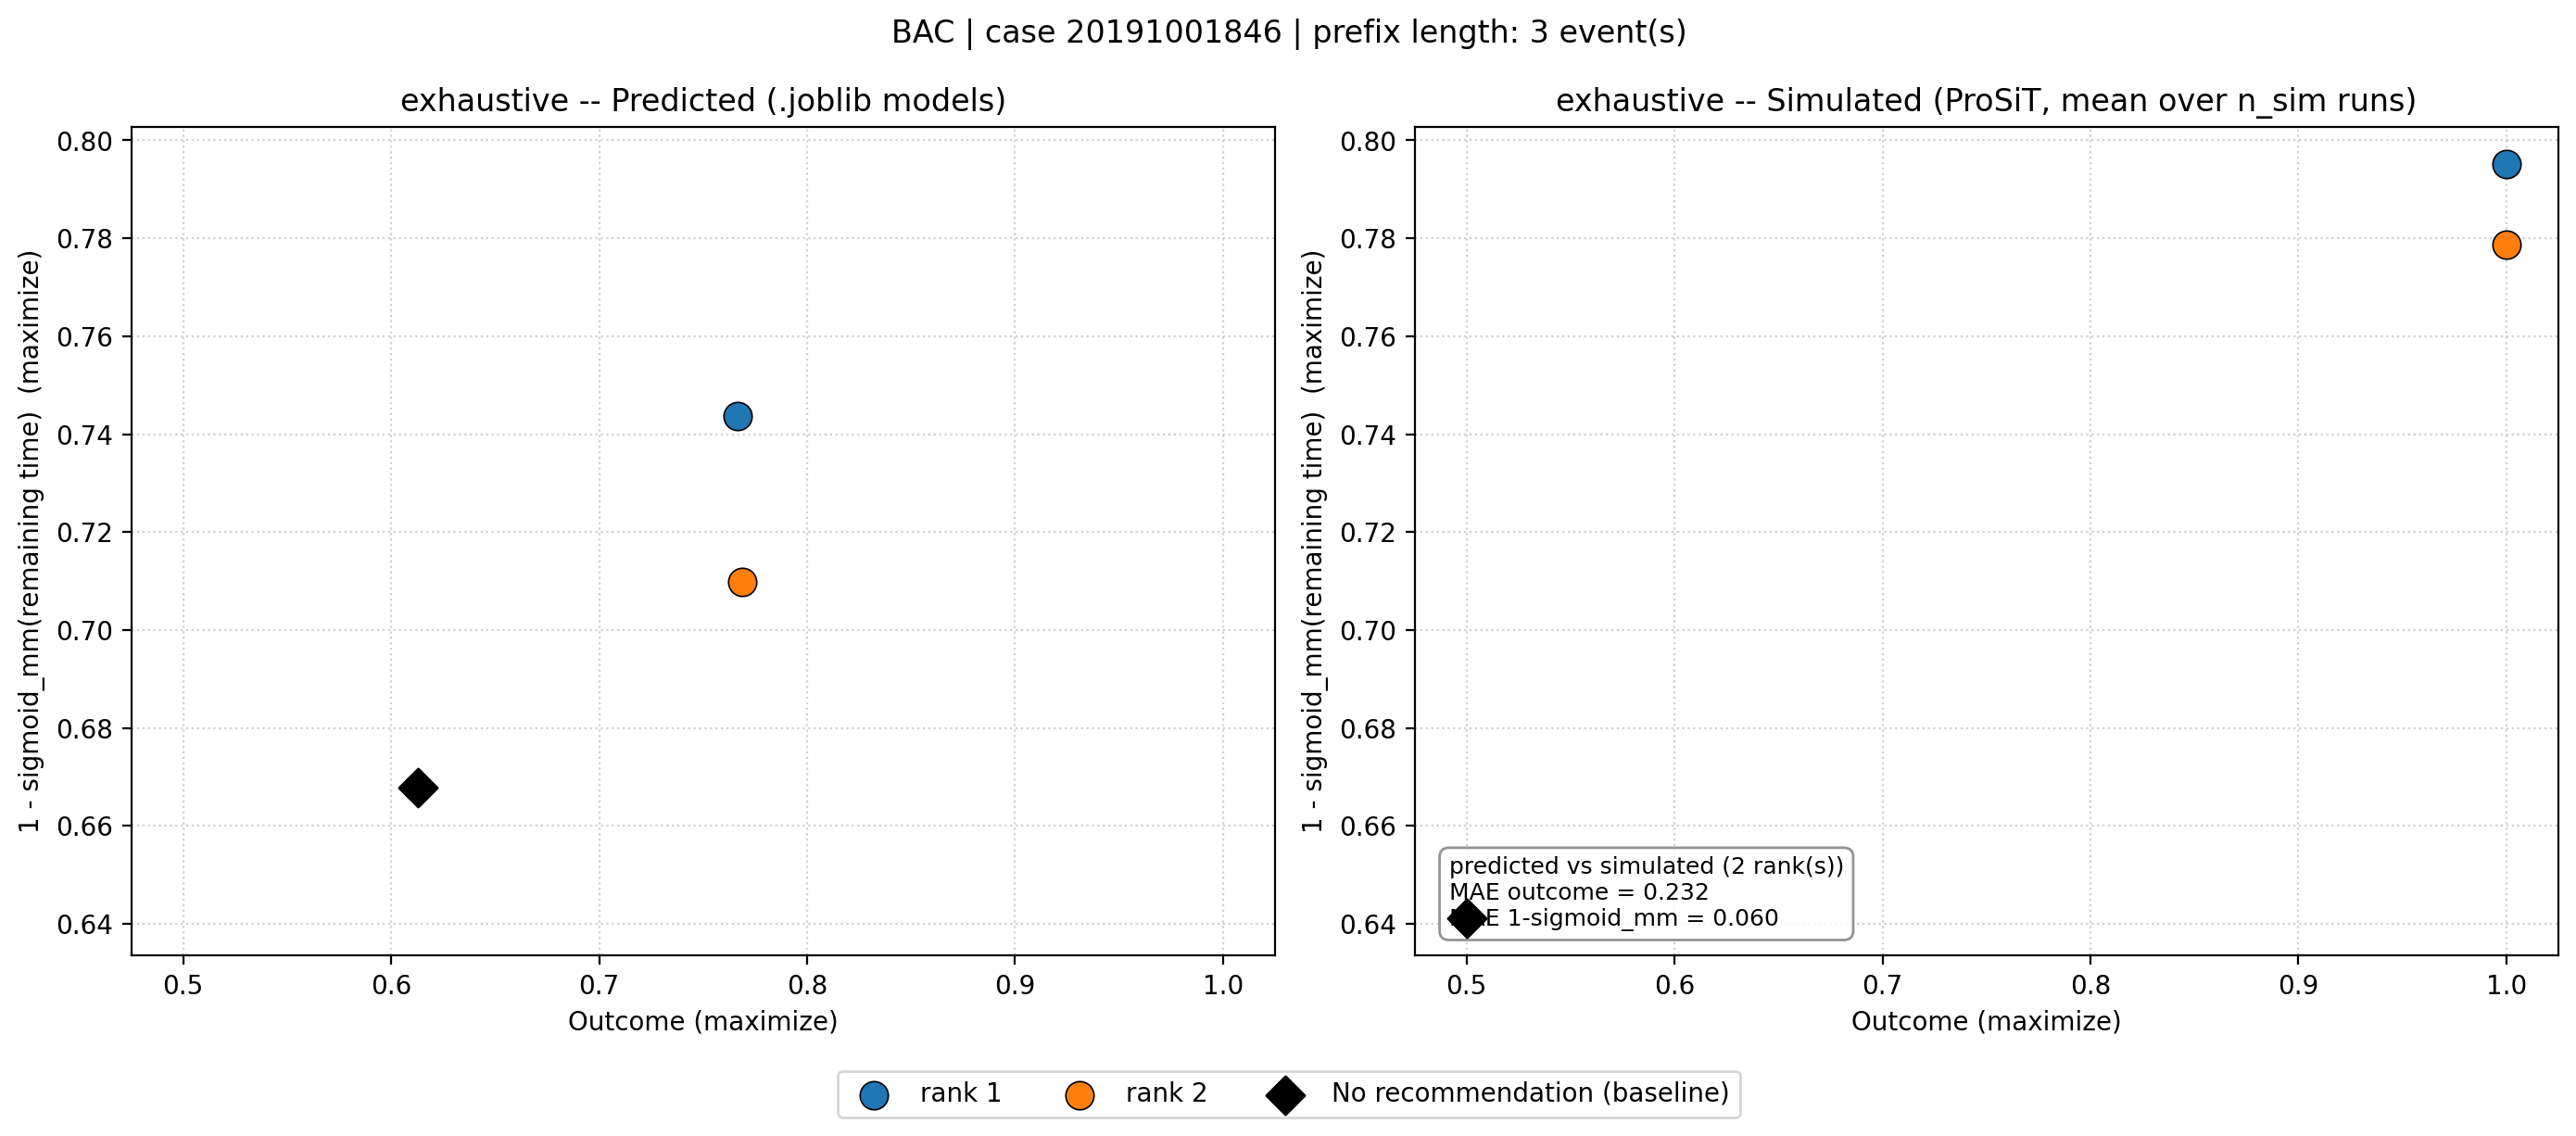
\includegraphics[width=\linewidth]{predicted_vs_simulated/BAC_plots/BAC_20191001846_exhaustive_predicted_vs_simulated.png}
    \end{minipage}
    \hfill
    \begin{minipage}{0.45\textwidth}
        \centering
        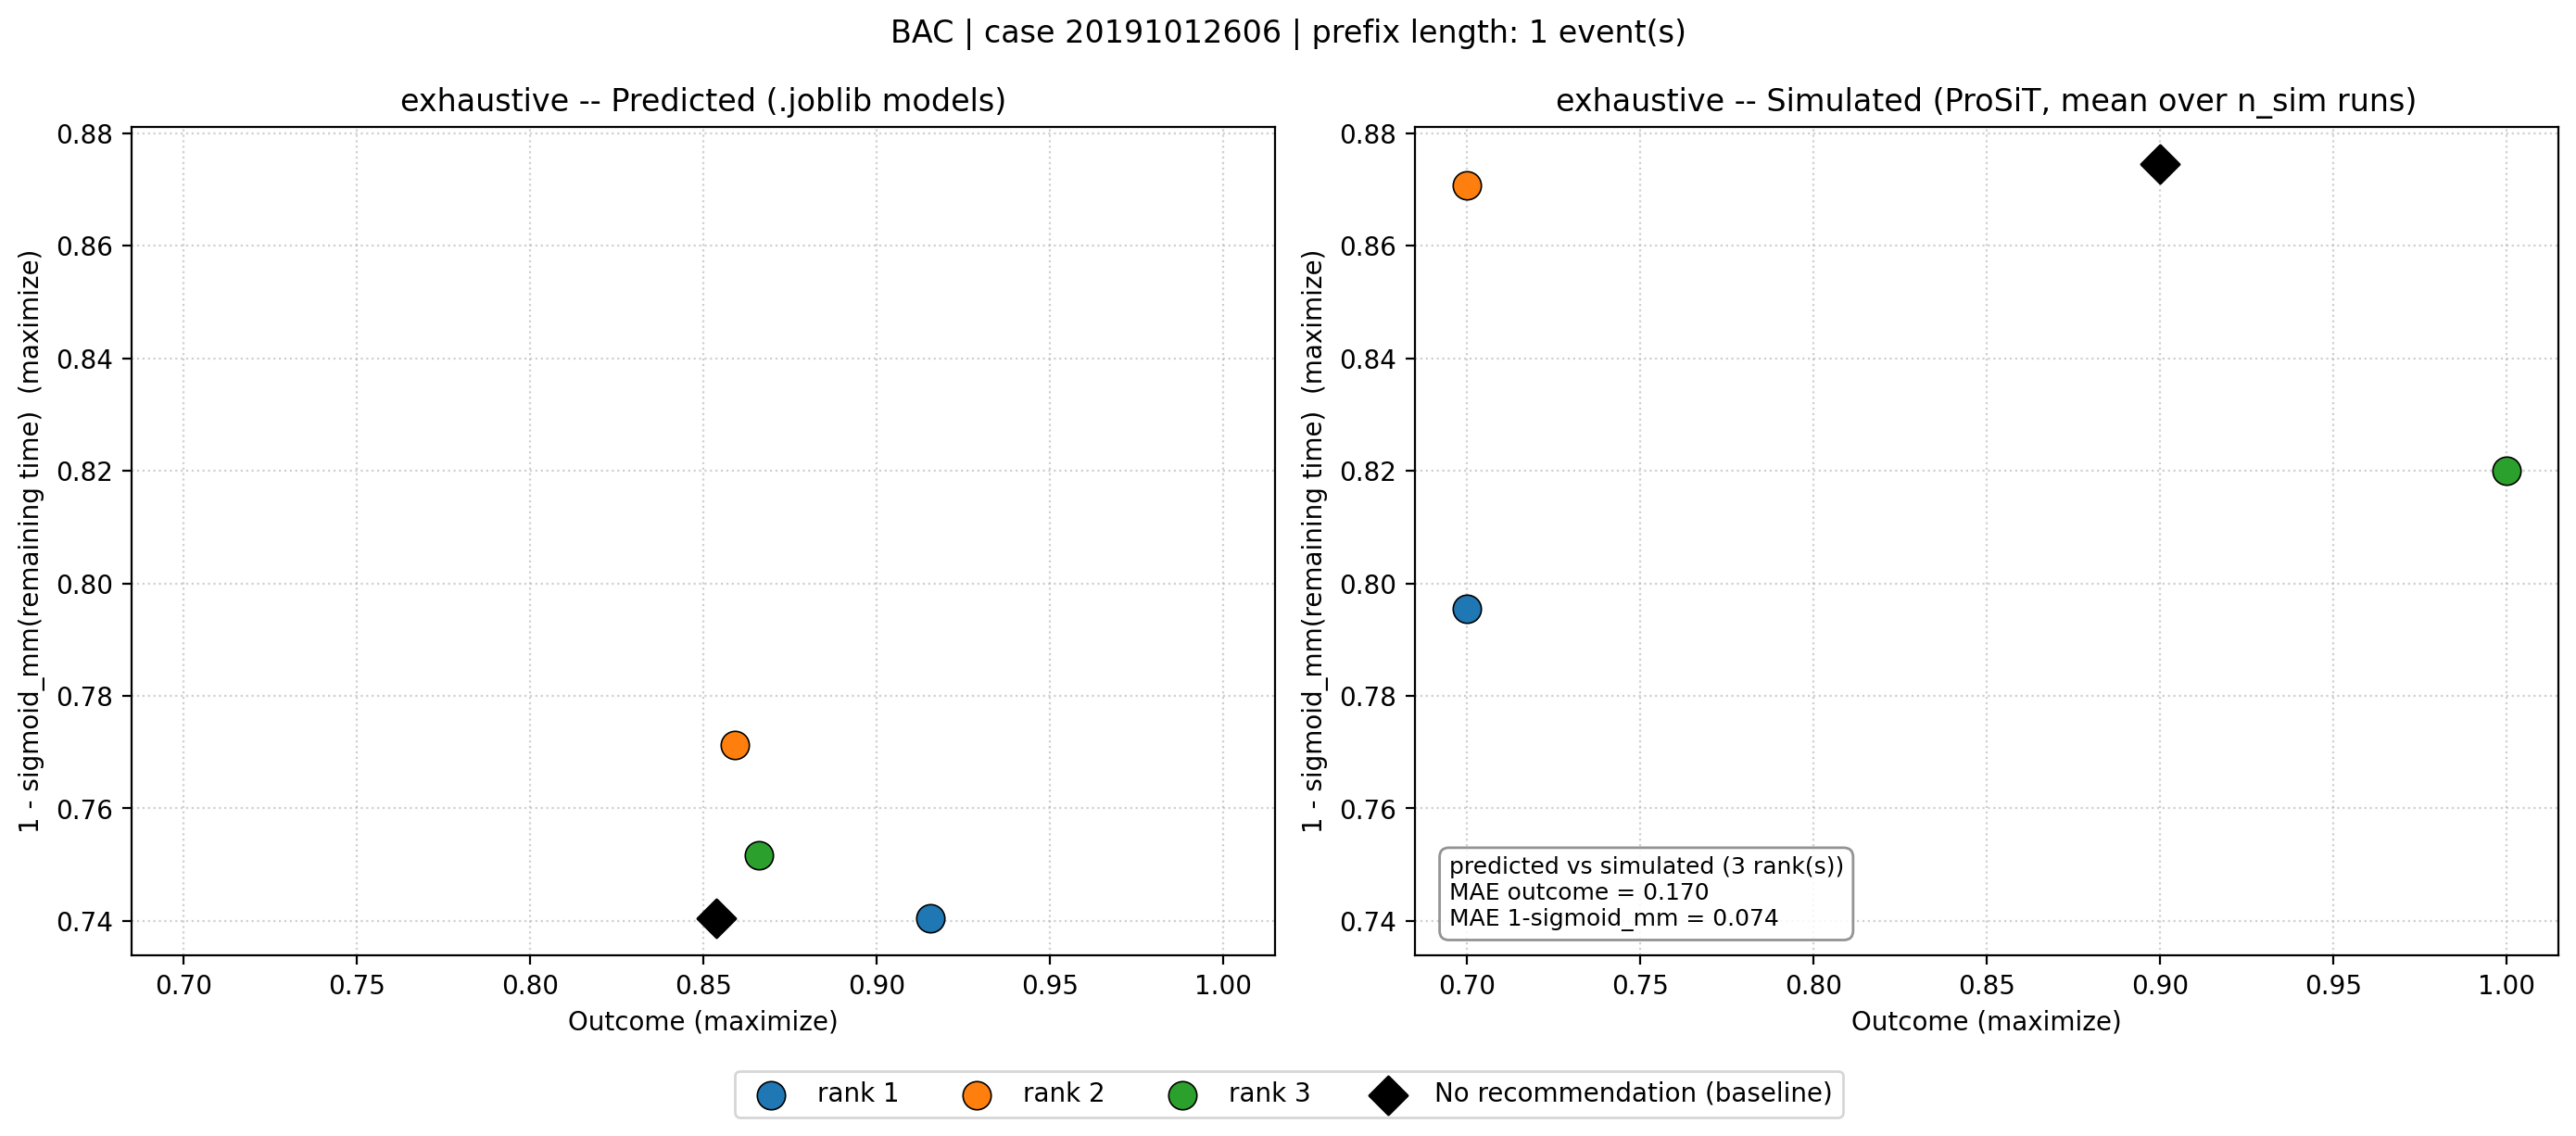
\includegraphics[width=\linewidth]{predicted_vs_simulated/BAC_plots/BAC_20191012606_exhaustive_predicted_vs_simulated.png}
    \end{minipage}
    \vspace{0.4cm}
    \begin{minipage}{0.45\textwidth}
        \centering
        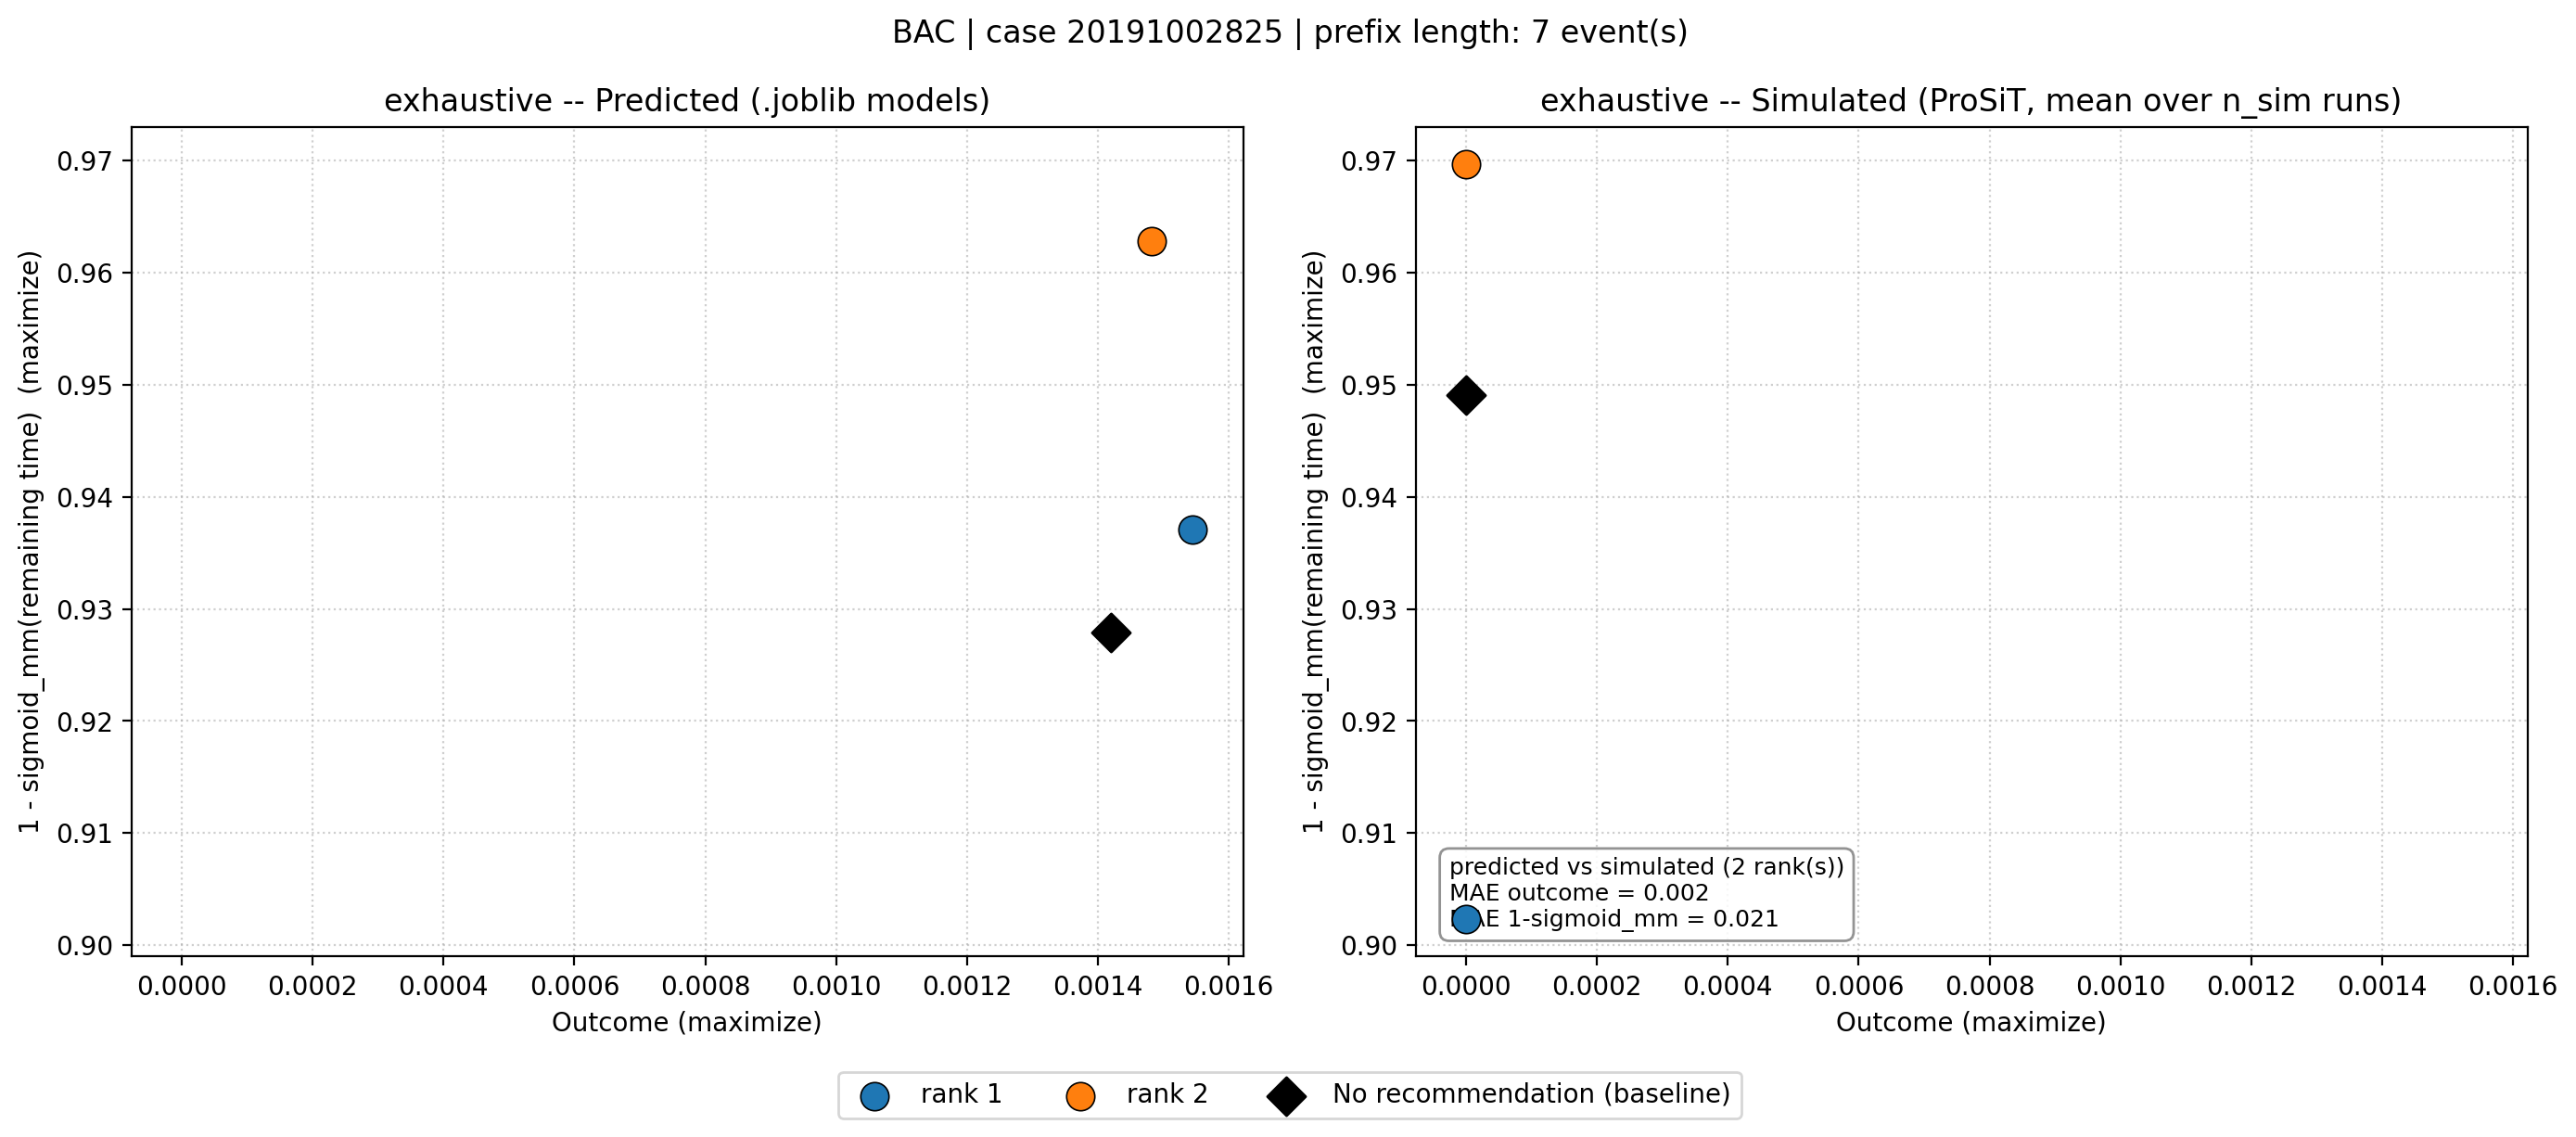
\includegraphics[width=\linewidth]{predicted_vs_simulated/BAC_plots/BAC_20191002825_exhaustive_predicted_vs_simulated.png}
    \end{minipage}
\end{frame}

\begin{frame}{Experimental Results: Predicted vs.\ Simulated (BPI12)}
    \centering
    \begin{minipage}{0.45\textwidth}
        \centering
        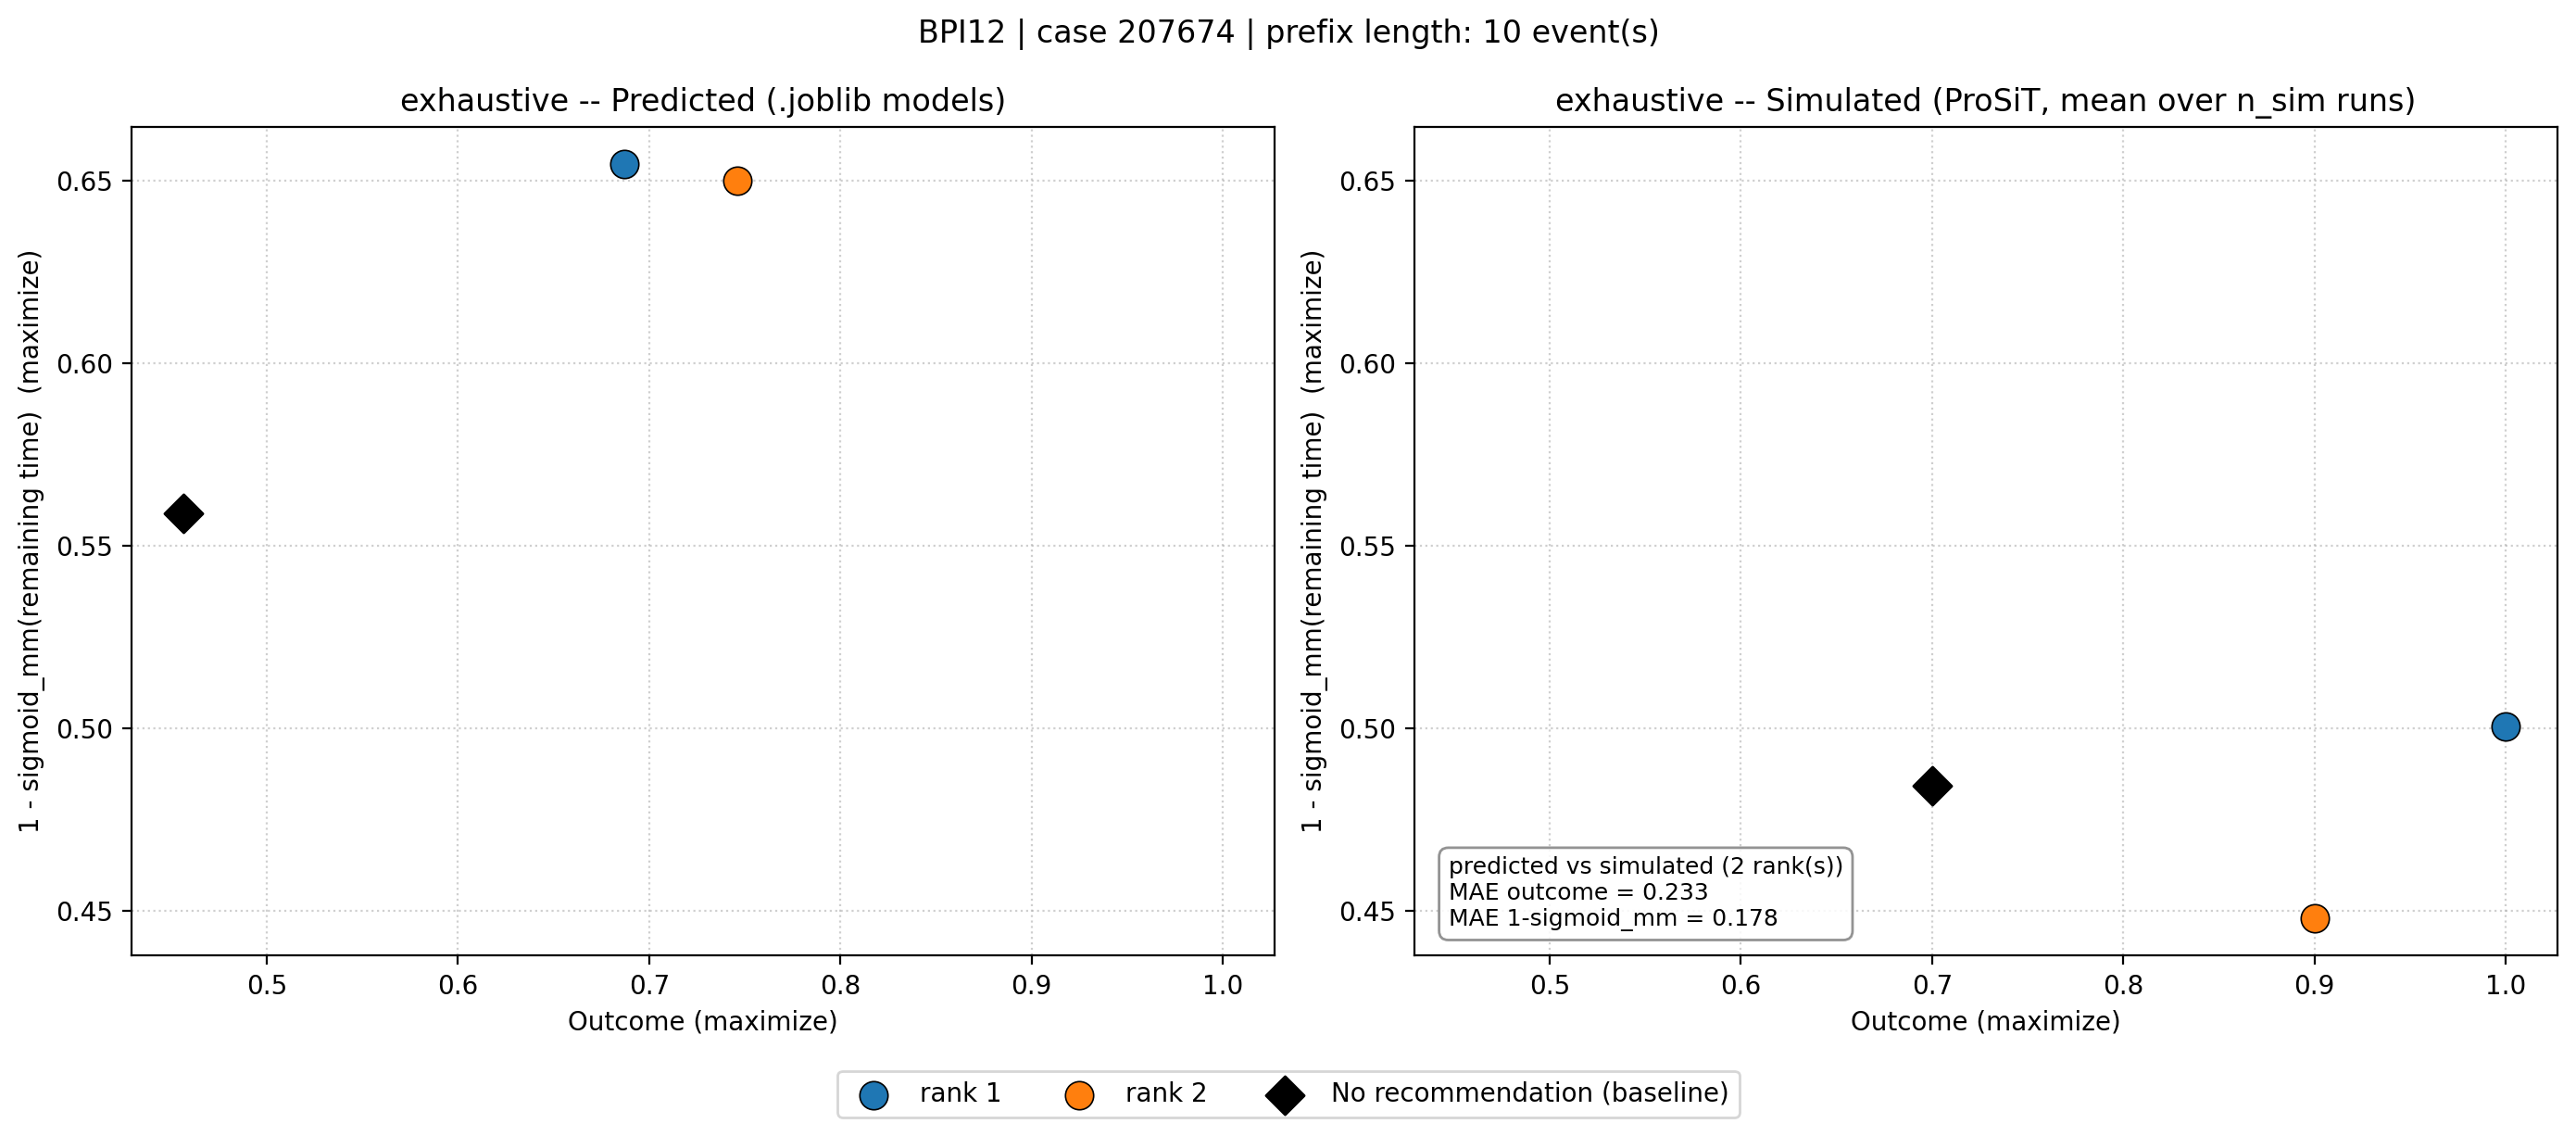
\includegraphics[width=\linewidth]{predicted_vs_simulated/BPI12_plots/BPI12_207674_exhaustive_predicted_vs_simulated.png}
    \end{minipage}
    \hfill
    \begin{minipage}{0.45\textwidth}
        \centering
        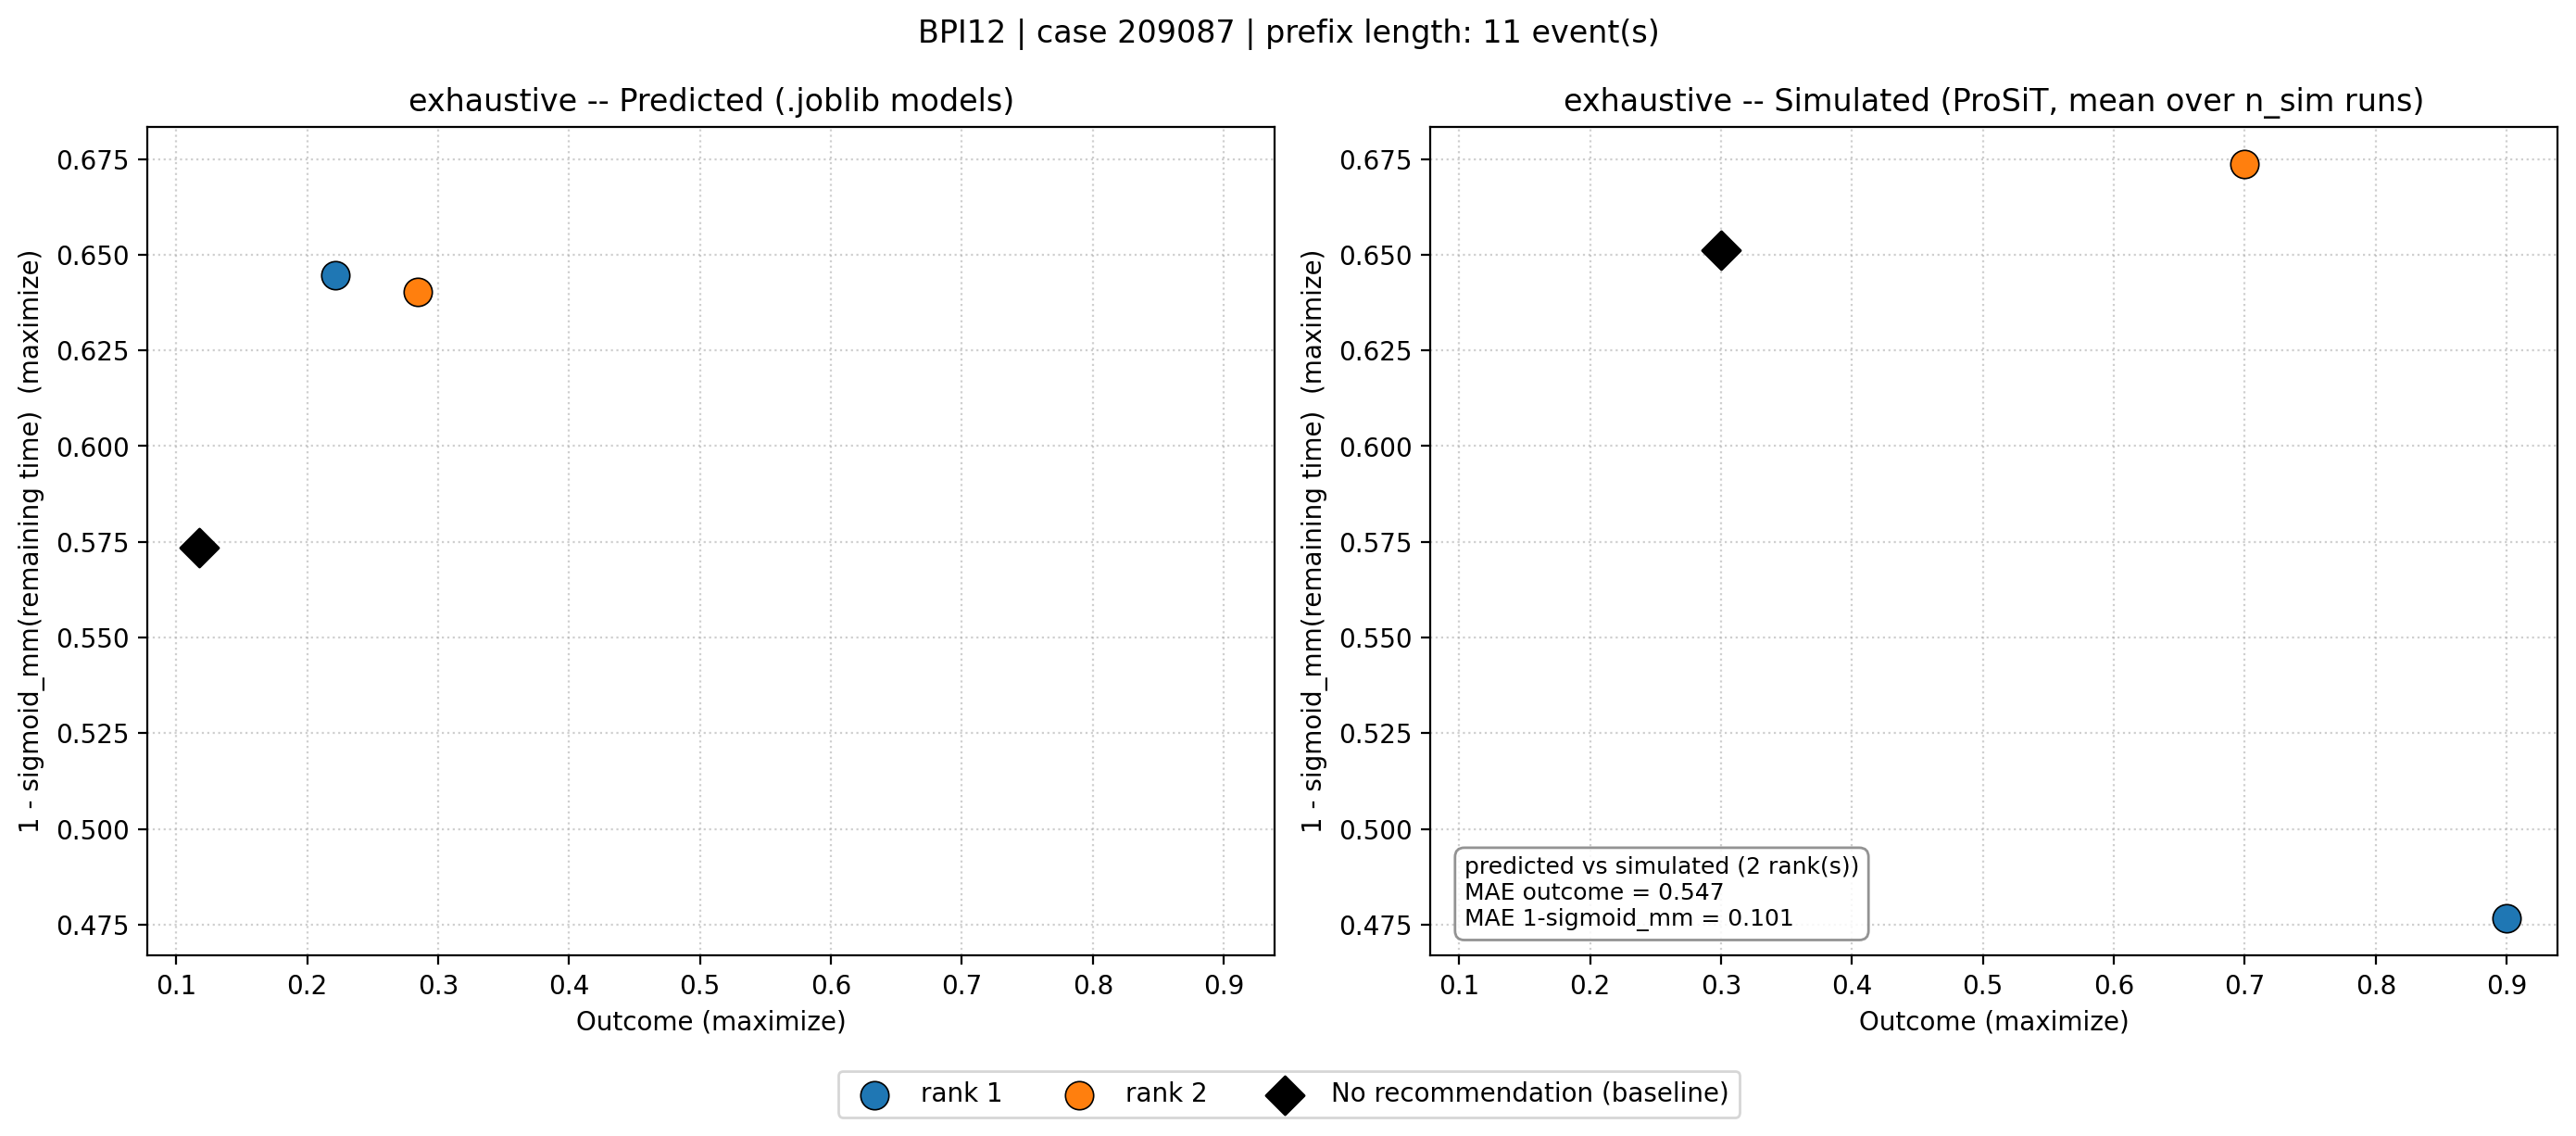
\includegraphics[width=\linewidth]{predicted_vs_simulated/BPI12_plots/BPI12_209087_exhaustive_predicted_vs_simulated.png}
    \end{minipage}
    \vspace{0.4cm}
    \begin{minipage}{0.45\textwidth}
        \centering
        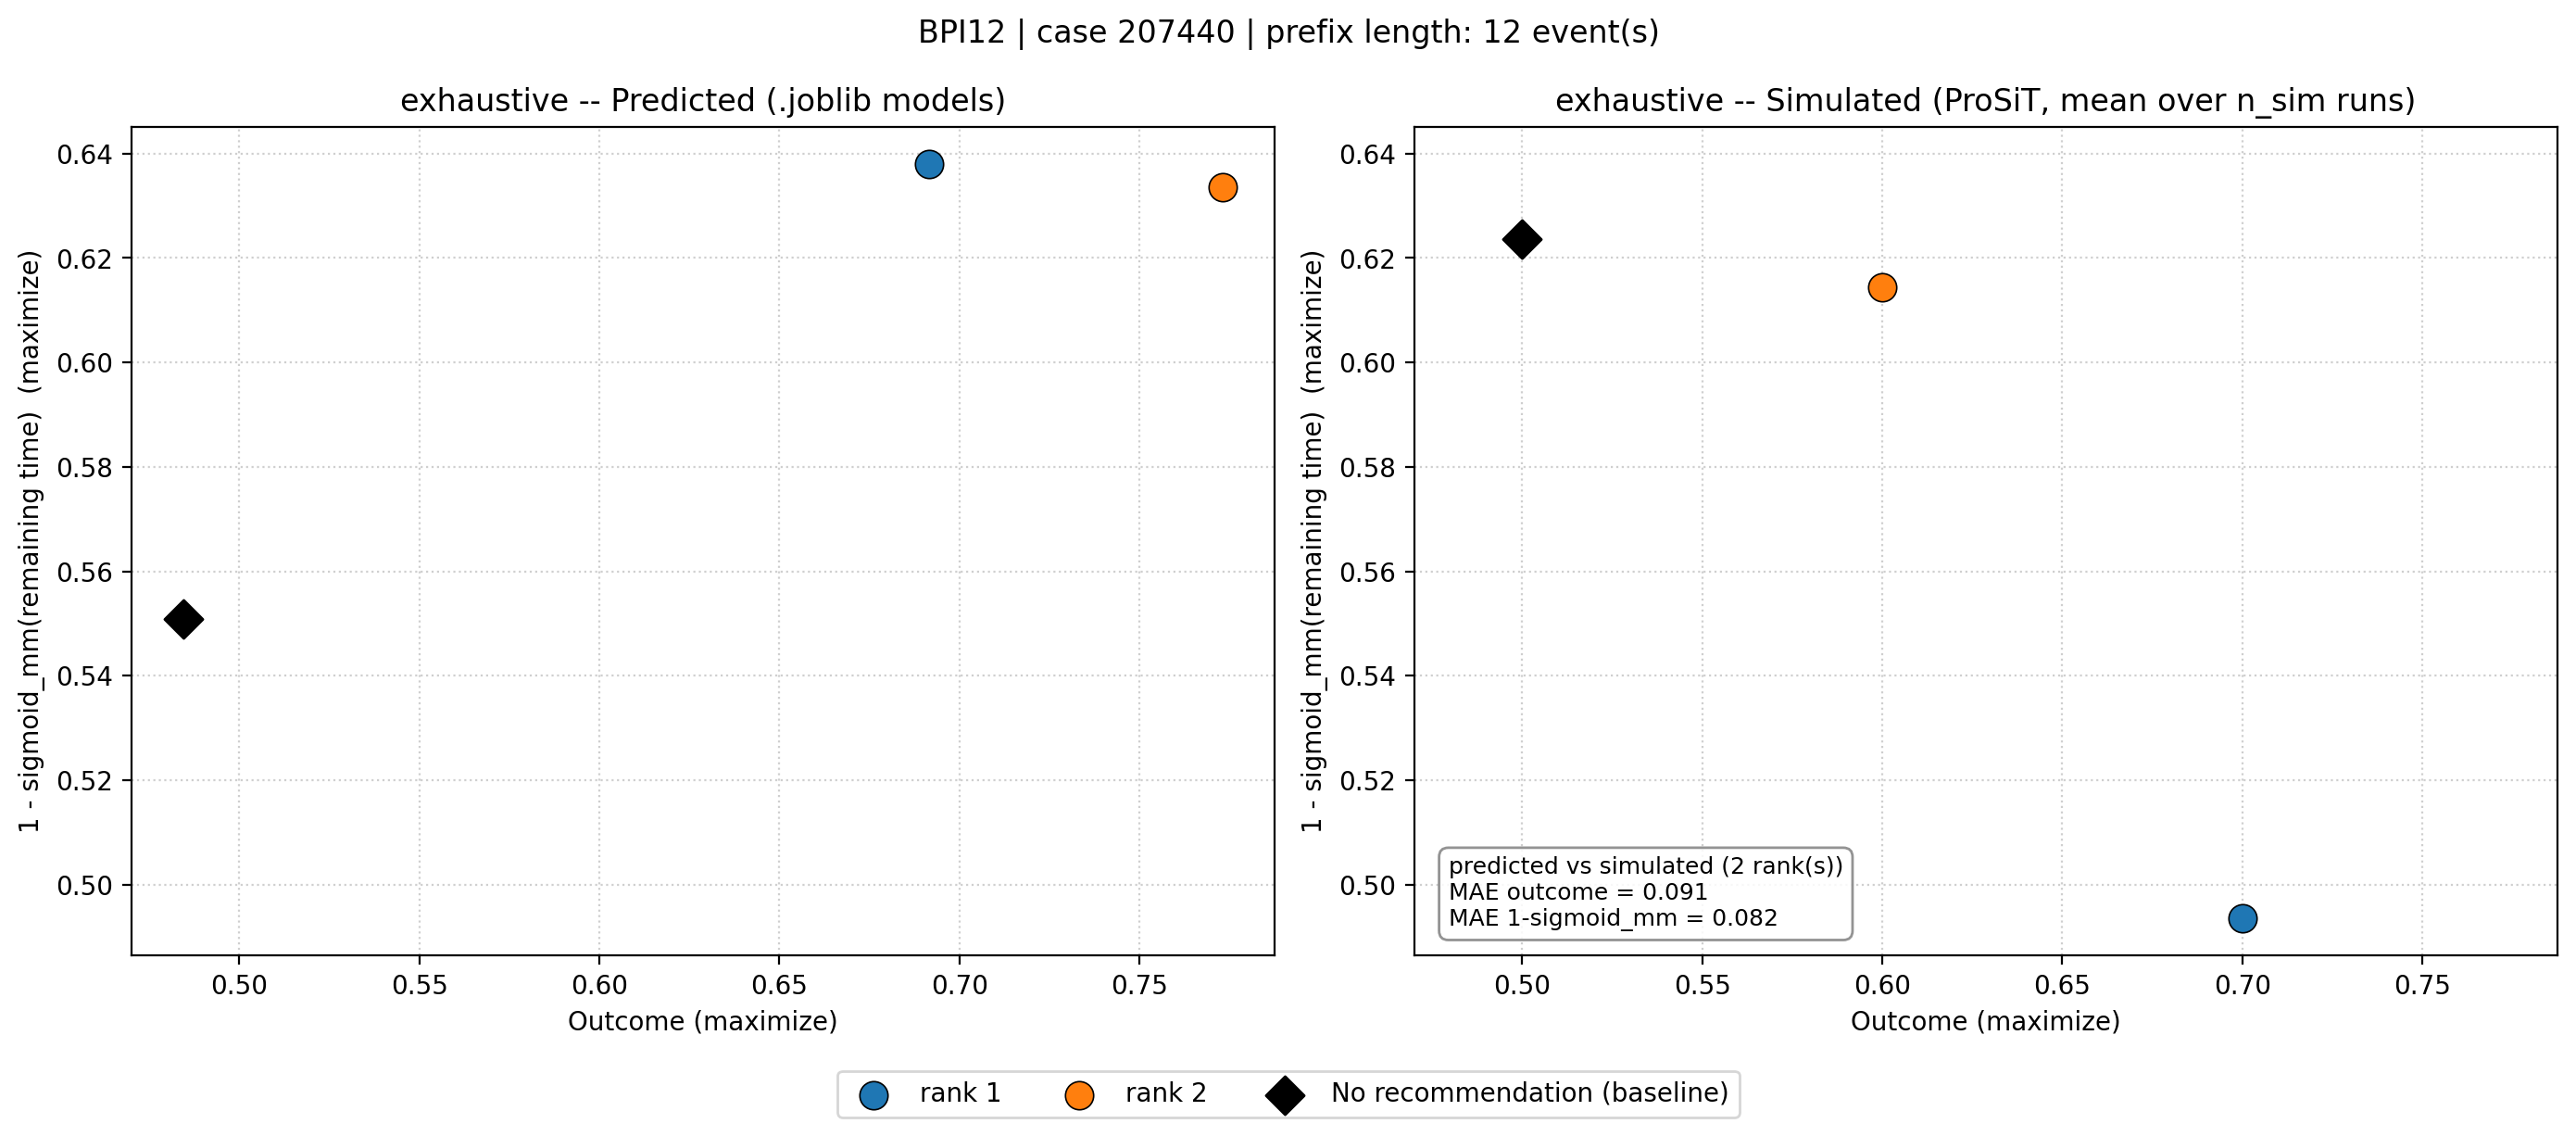
\includegraphics[width=\linewidth]{predicted_vs_simulated/BPI12_plots/BPI12_207440_exhaustive_predicted_vs_simulated.png}
    \end{minipage}
\end{frame}

\begin{frame}{Experimental Results: Predicted vs.\ Simulated (bpi17 before)}
    \centering
    \begin{minipage}{0.45\textwidth}
        \centering
        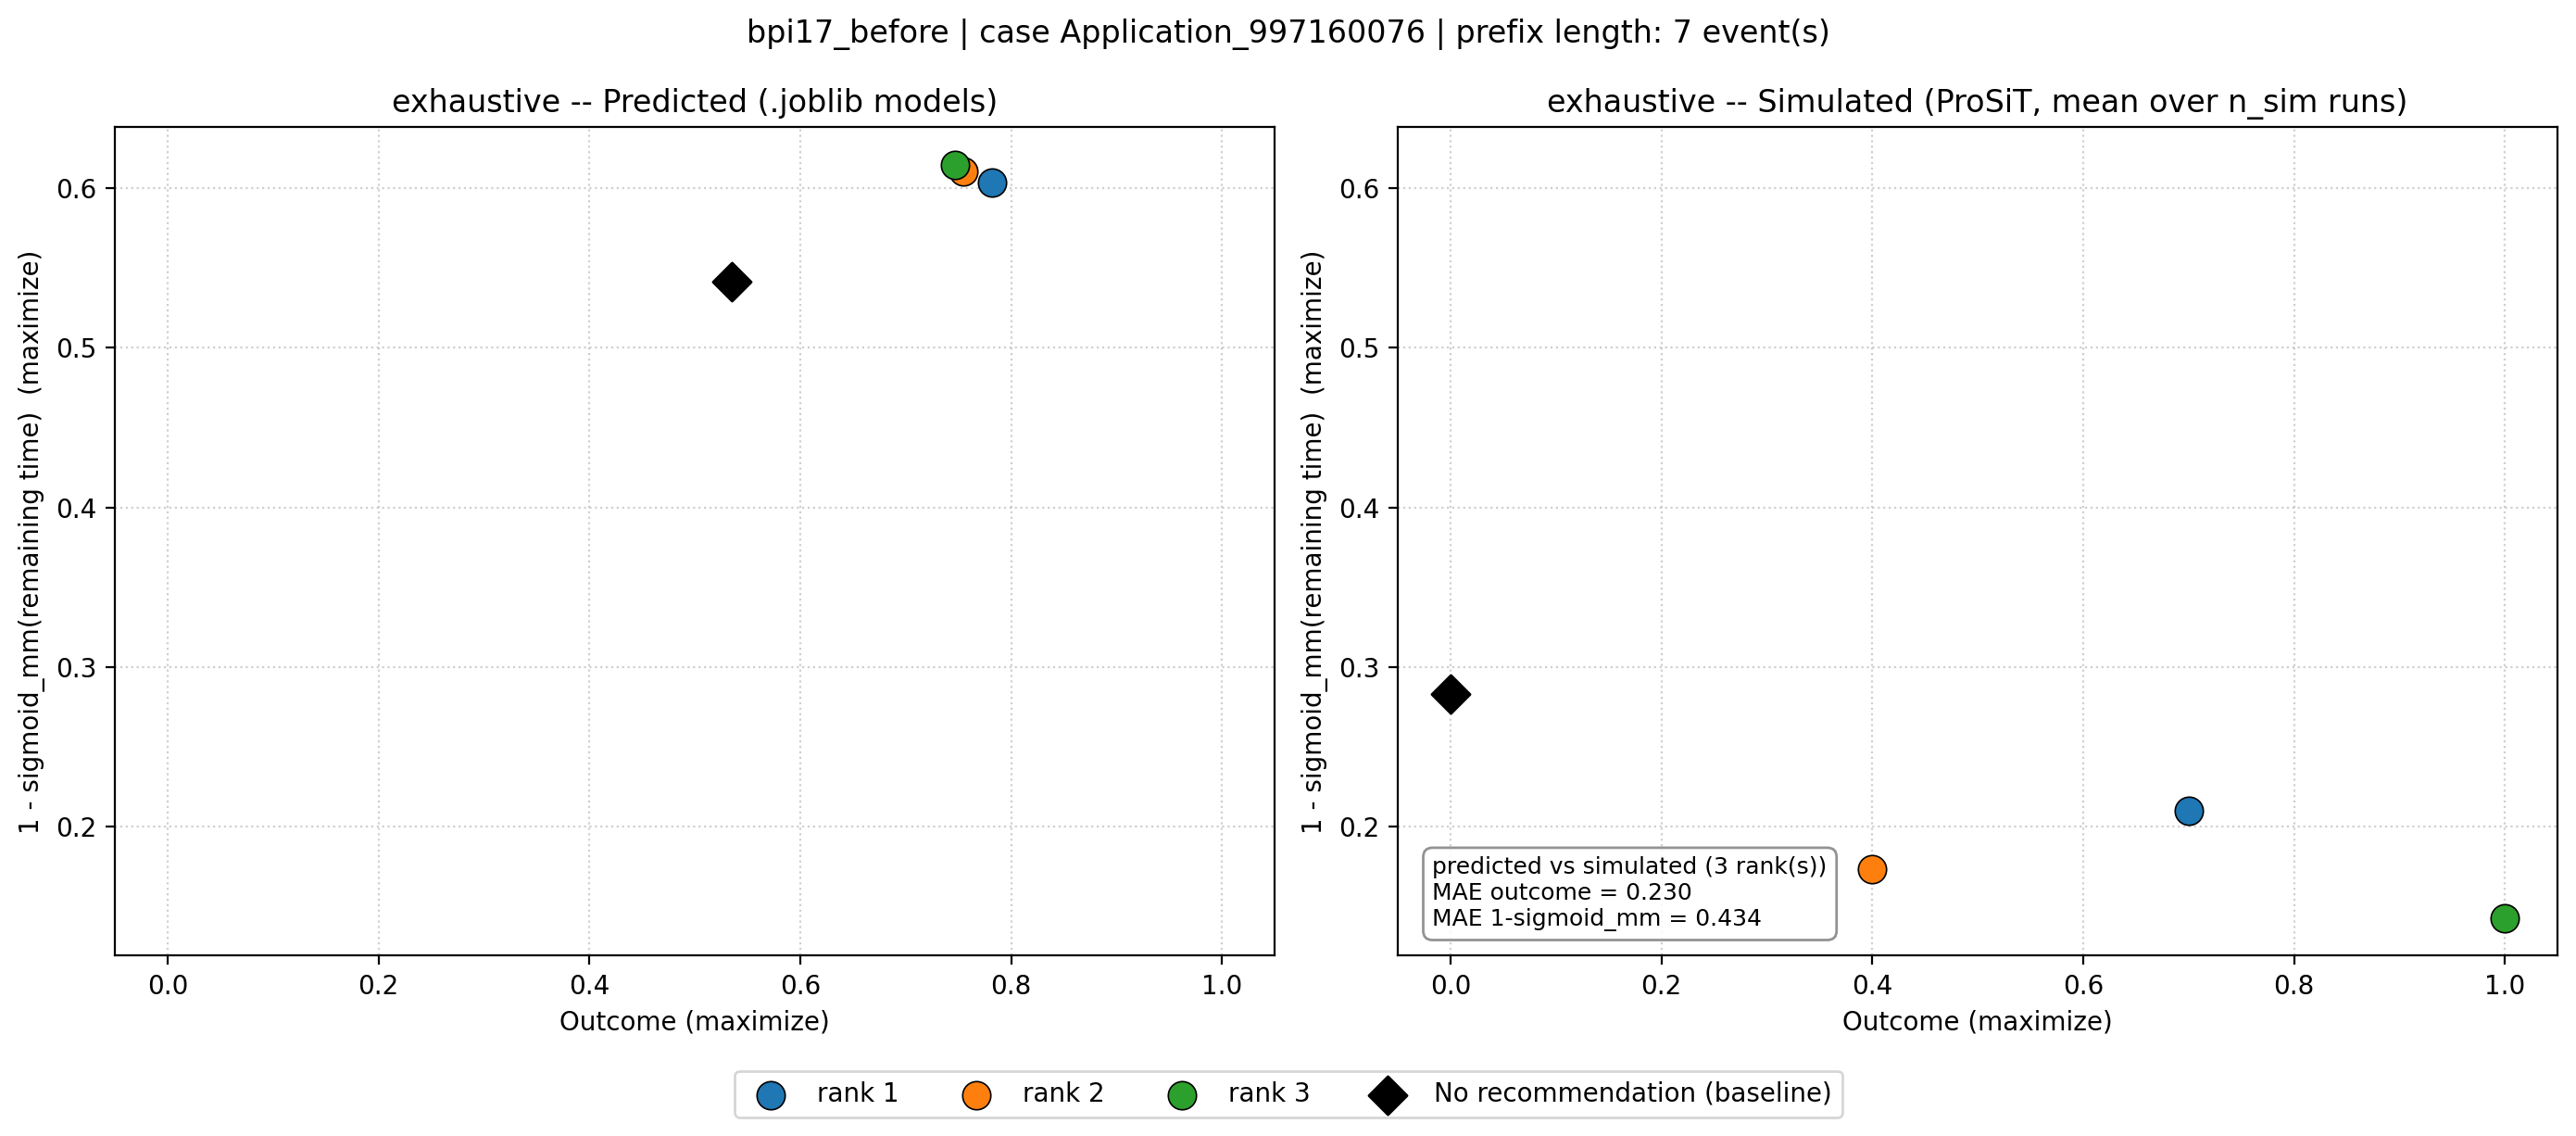
\includegraphics[width=\linewidth]{predicted_vs_simulated/bpi17_before_plots/bpi17_before_Application_997160076_exhaustive_predicted_vs_simulated.png}
    \end{minipage}
    \hfill
    \begin{minipage}{0.45\textwidth}
        \centering
        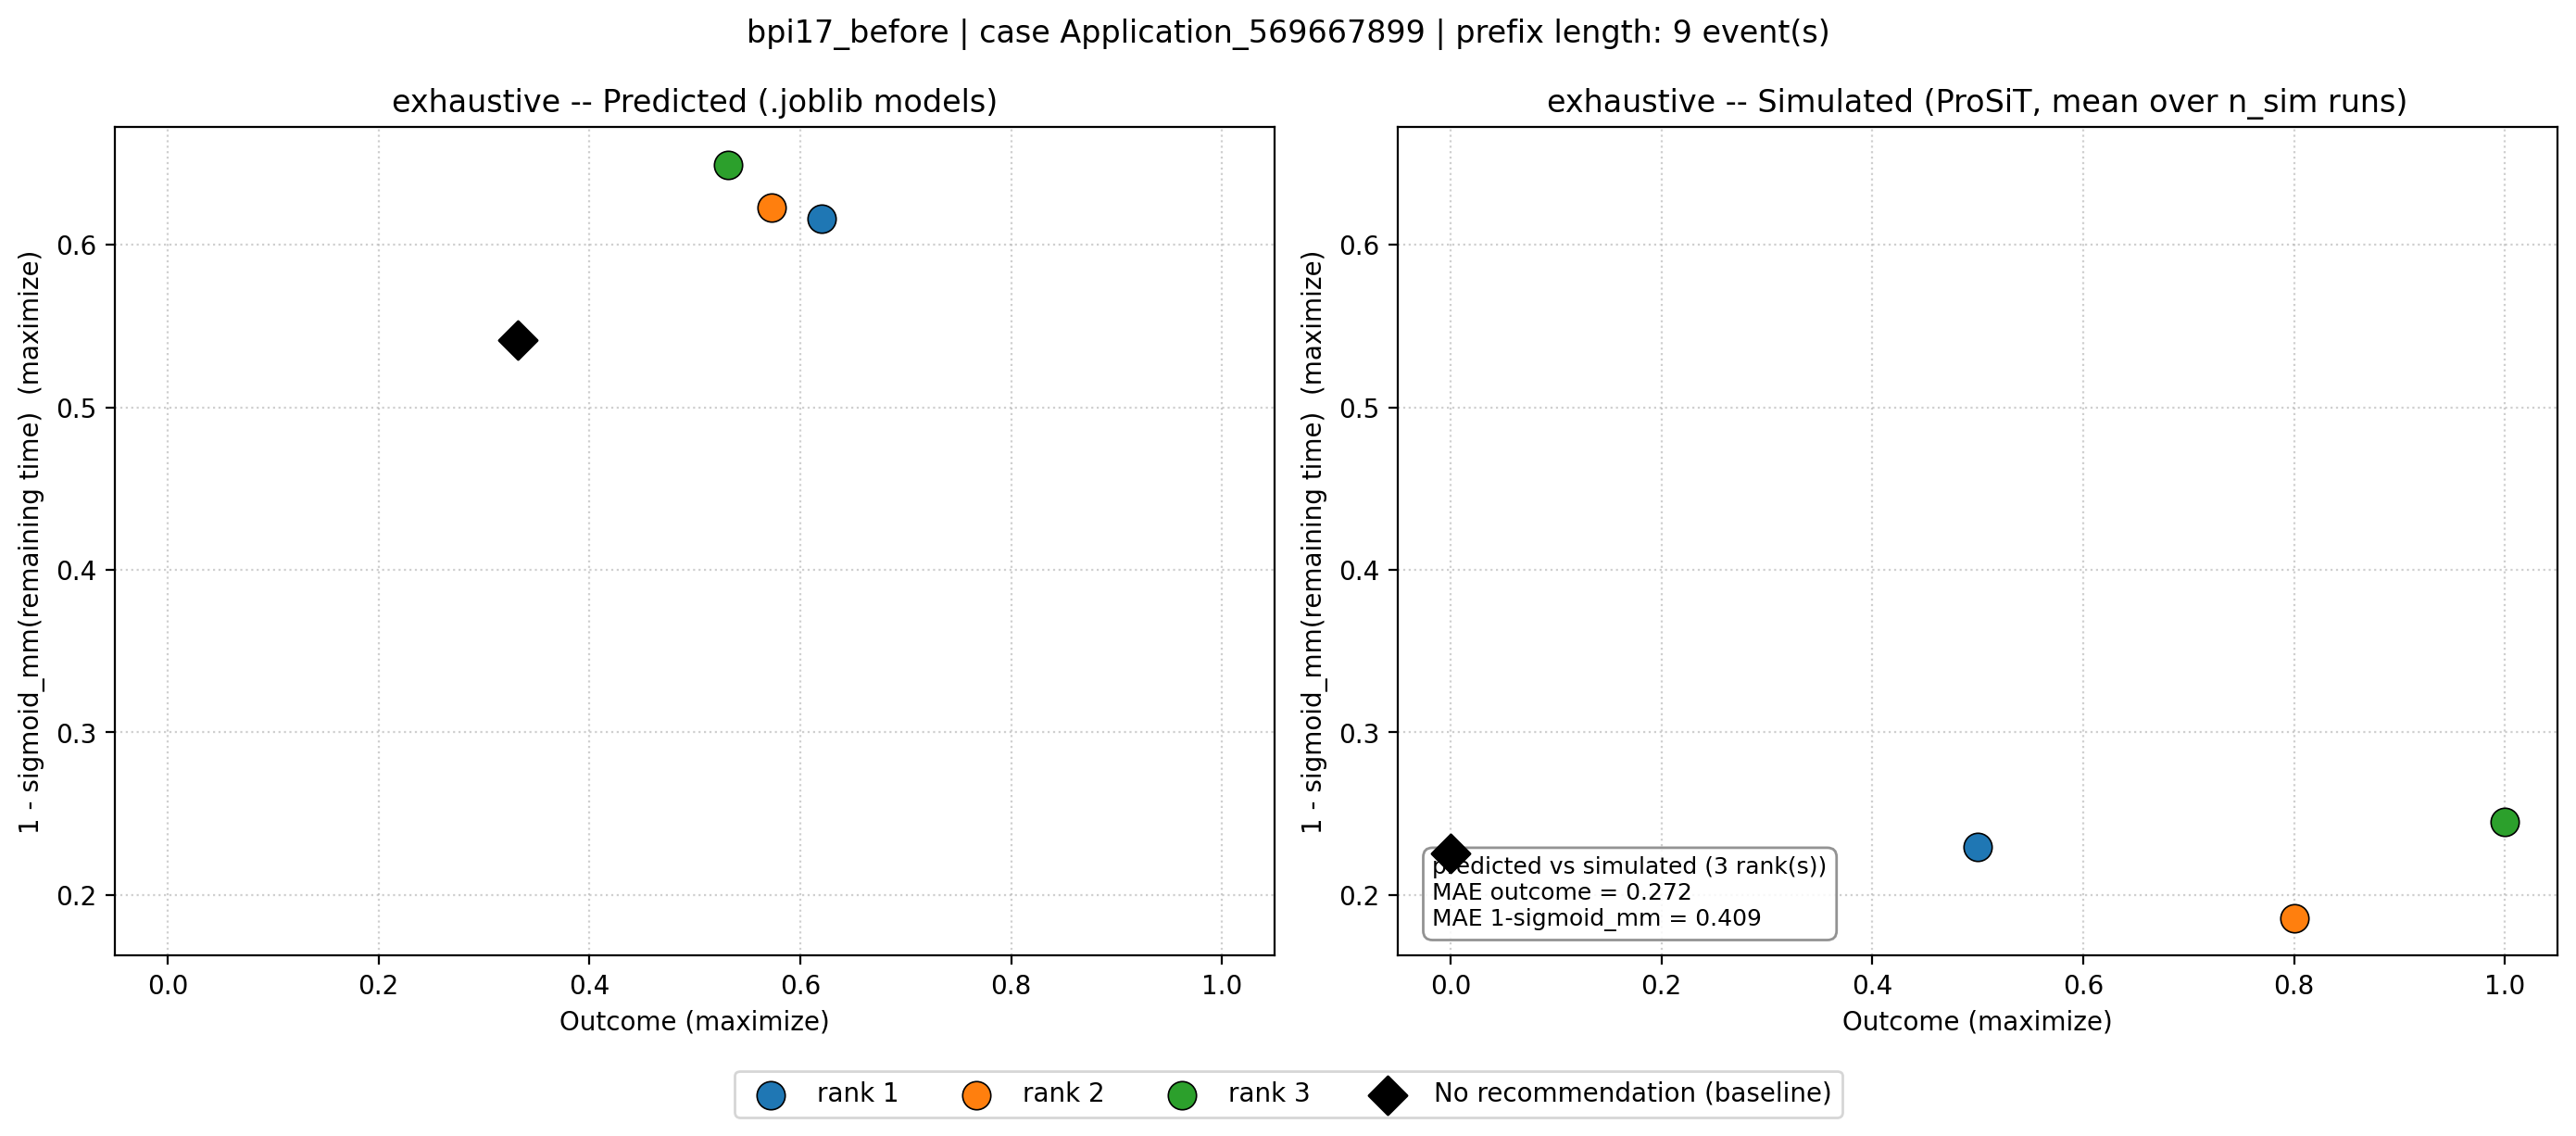
\includegraphics[width=\linewidth]{predicted_vs_simulated/bpi17_before_plots/bpi17_before_Application_569667899_exhaustive_predicted_vs_simulated.png}
    \end{minipage}
    \vspace{0.4cm}
    \begin{minipage}{0.45\textwidth}
        \centering
        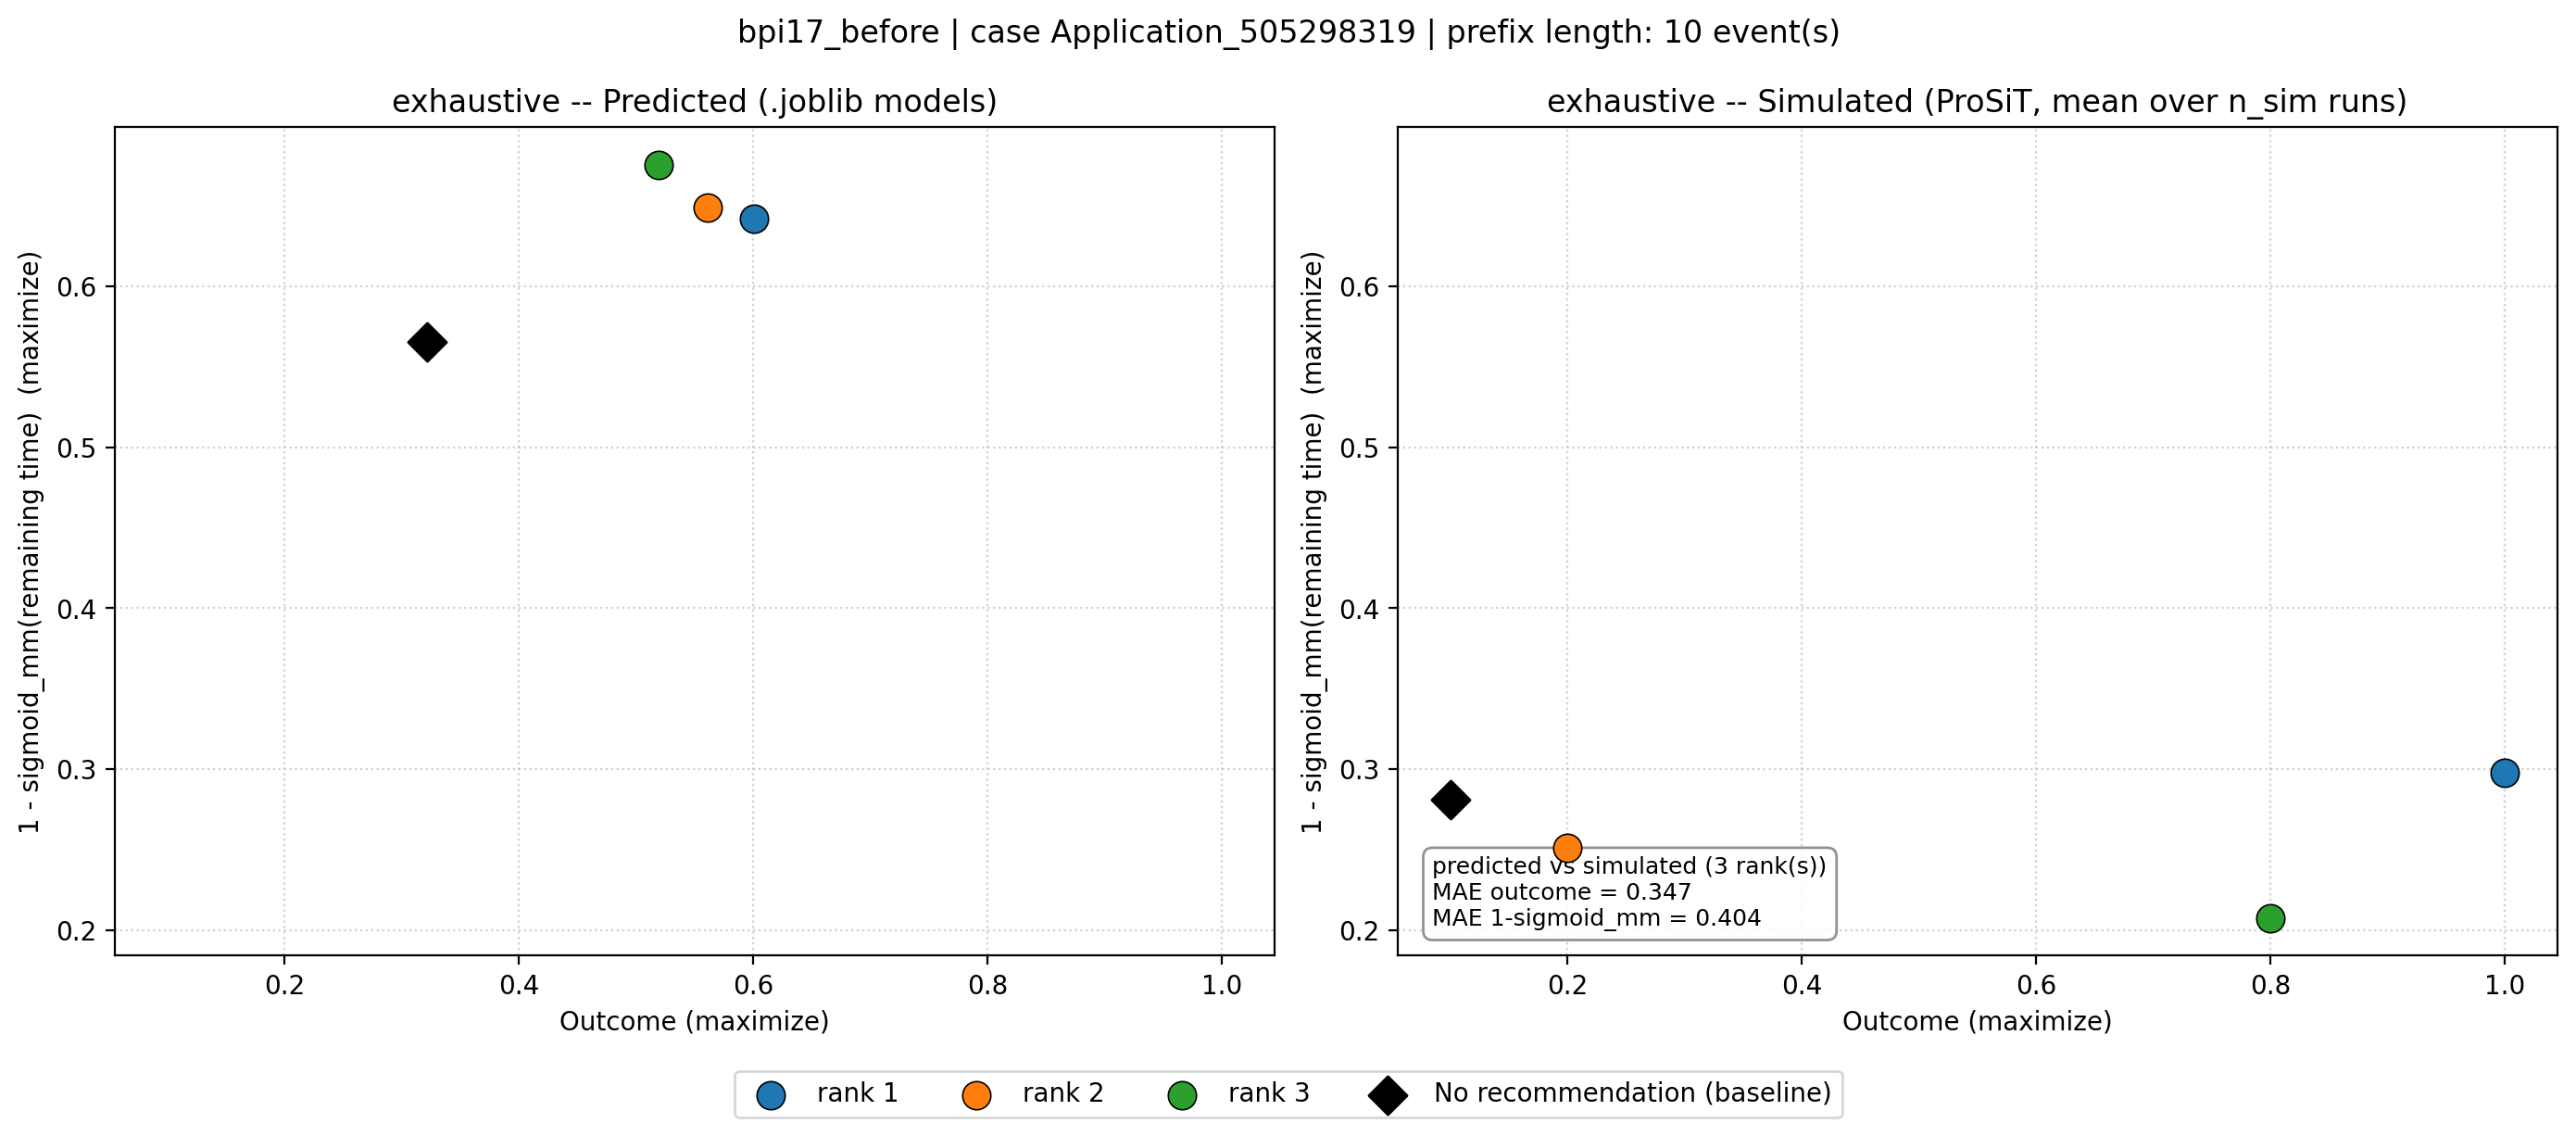
\includegraphics[width=\linewidth]{predicted_vs_simulated/bpi17_before_plots/bpi17_before_Application_505298319_exhaustive_predicted_vs_simulated.png}
    \end{minipage}
\end{frame}

\begin{frame}{Experimental Results: Predicted vs.\ Simulated (bpi17 after)}
    \centering
    \begin{minipage}{0.45\textwidth}
        \centering
        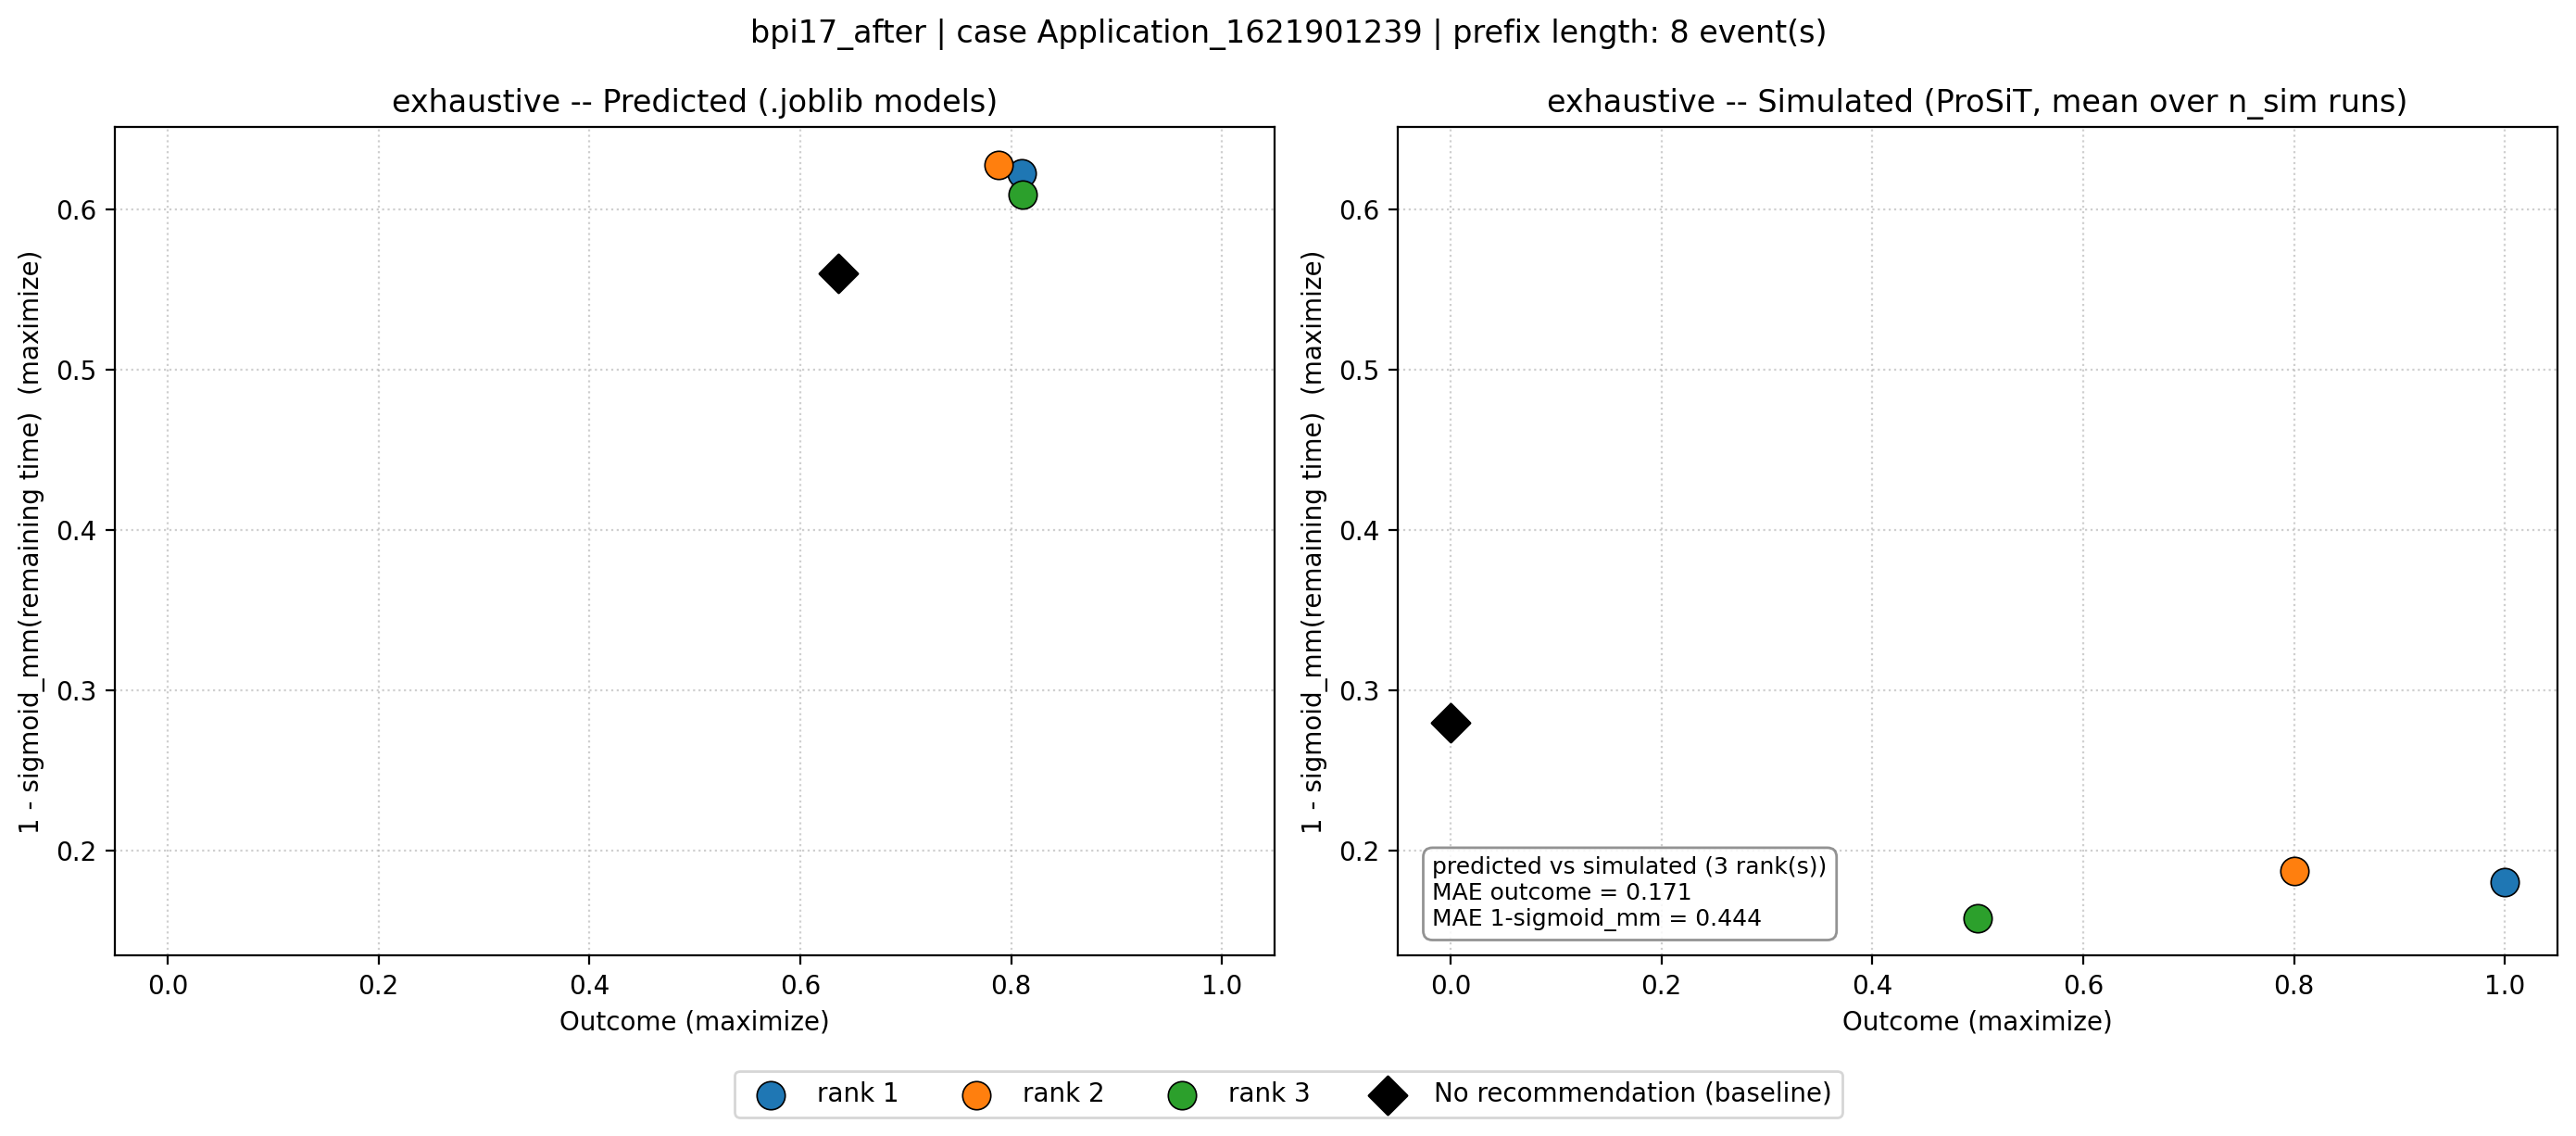
\includegraphics[width=\linewidth]{predicted_vs_simulated/bpi17_after_plots/bpi17_after_Application_1621901239_exhaustive_predicted_vs_simulated.png}
    \end{minipage}
    \hfill
    \begin{minipage}{0.45\textwidth}
        \centering
        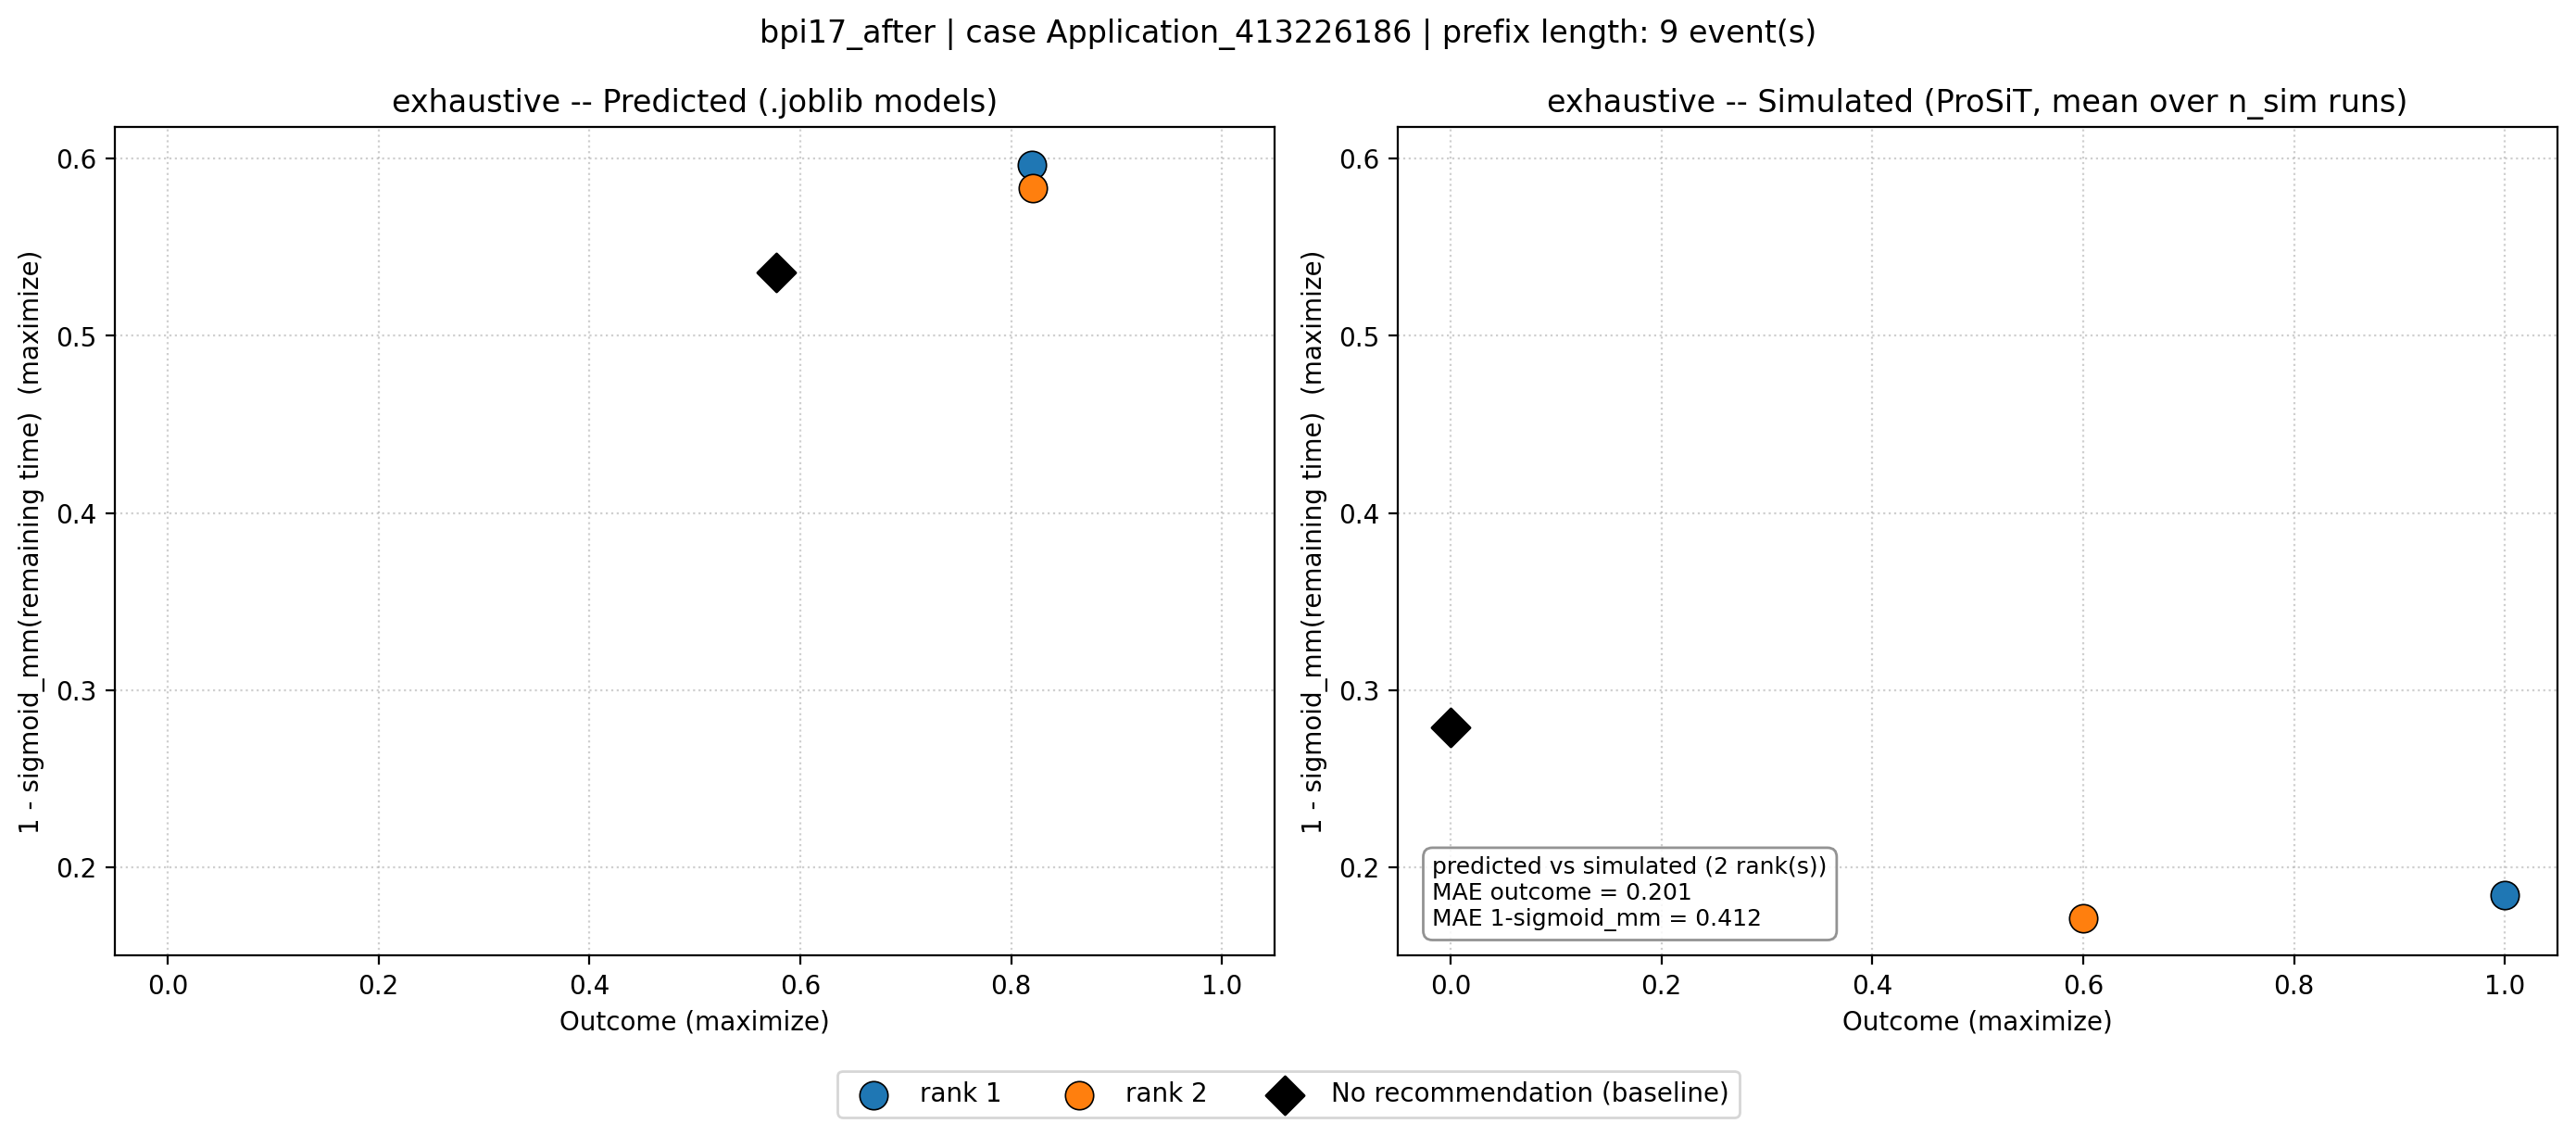
\includegraphics[width=\linewidth]{predicted_vs_simulated/bpi17_after_plots/bpi17_after_Application_413226186_exhaustive_predicted_vs_simulated.png}
    \end{minipage}
    \vspace{0.4cm}
    \begin{minipage}{0.45\textwidth}
        \centering
        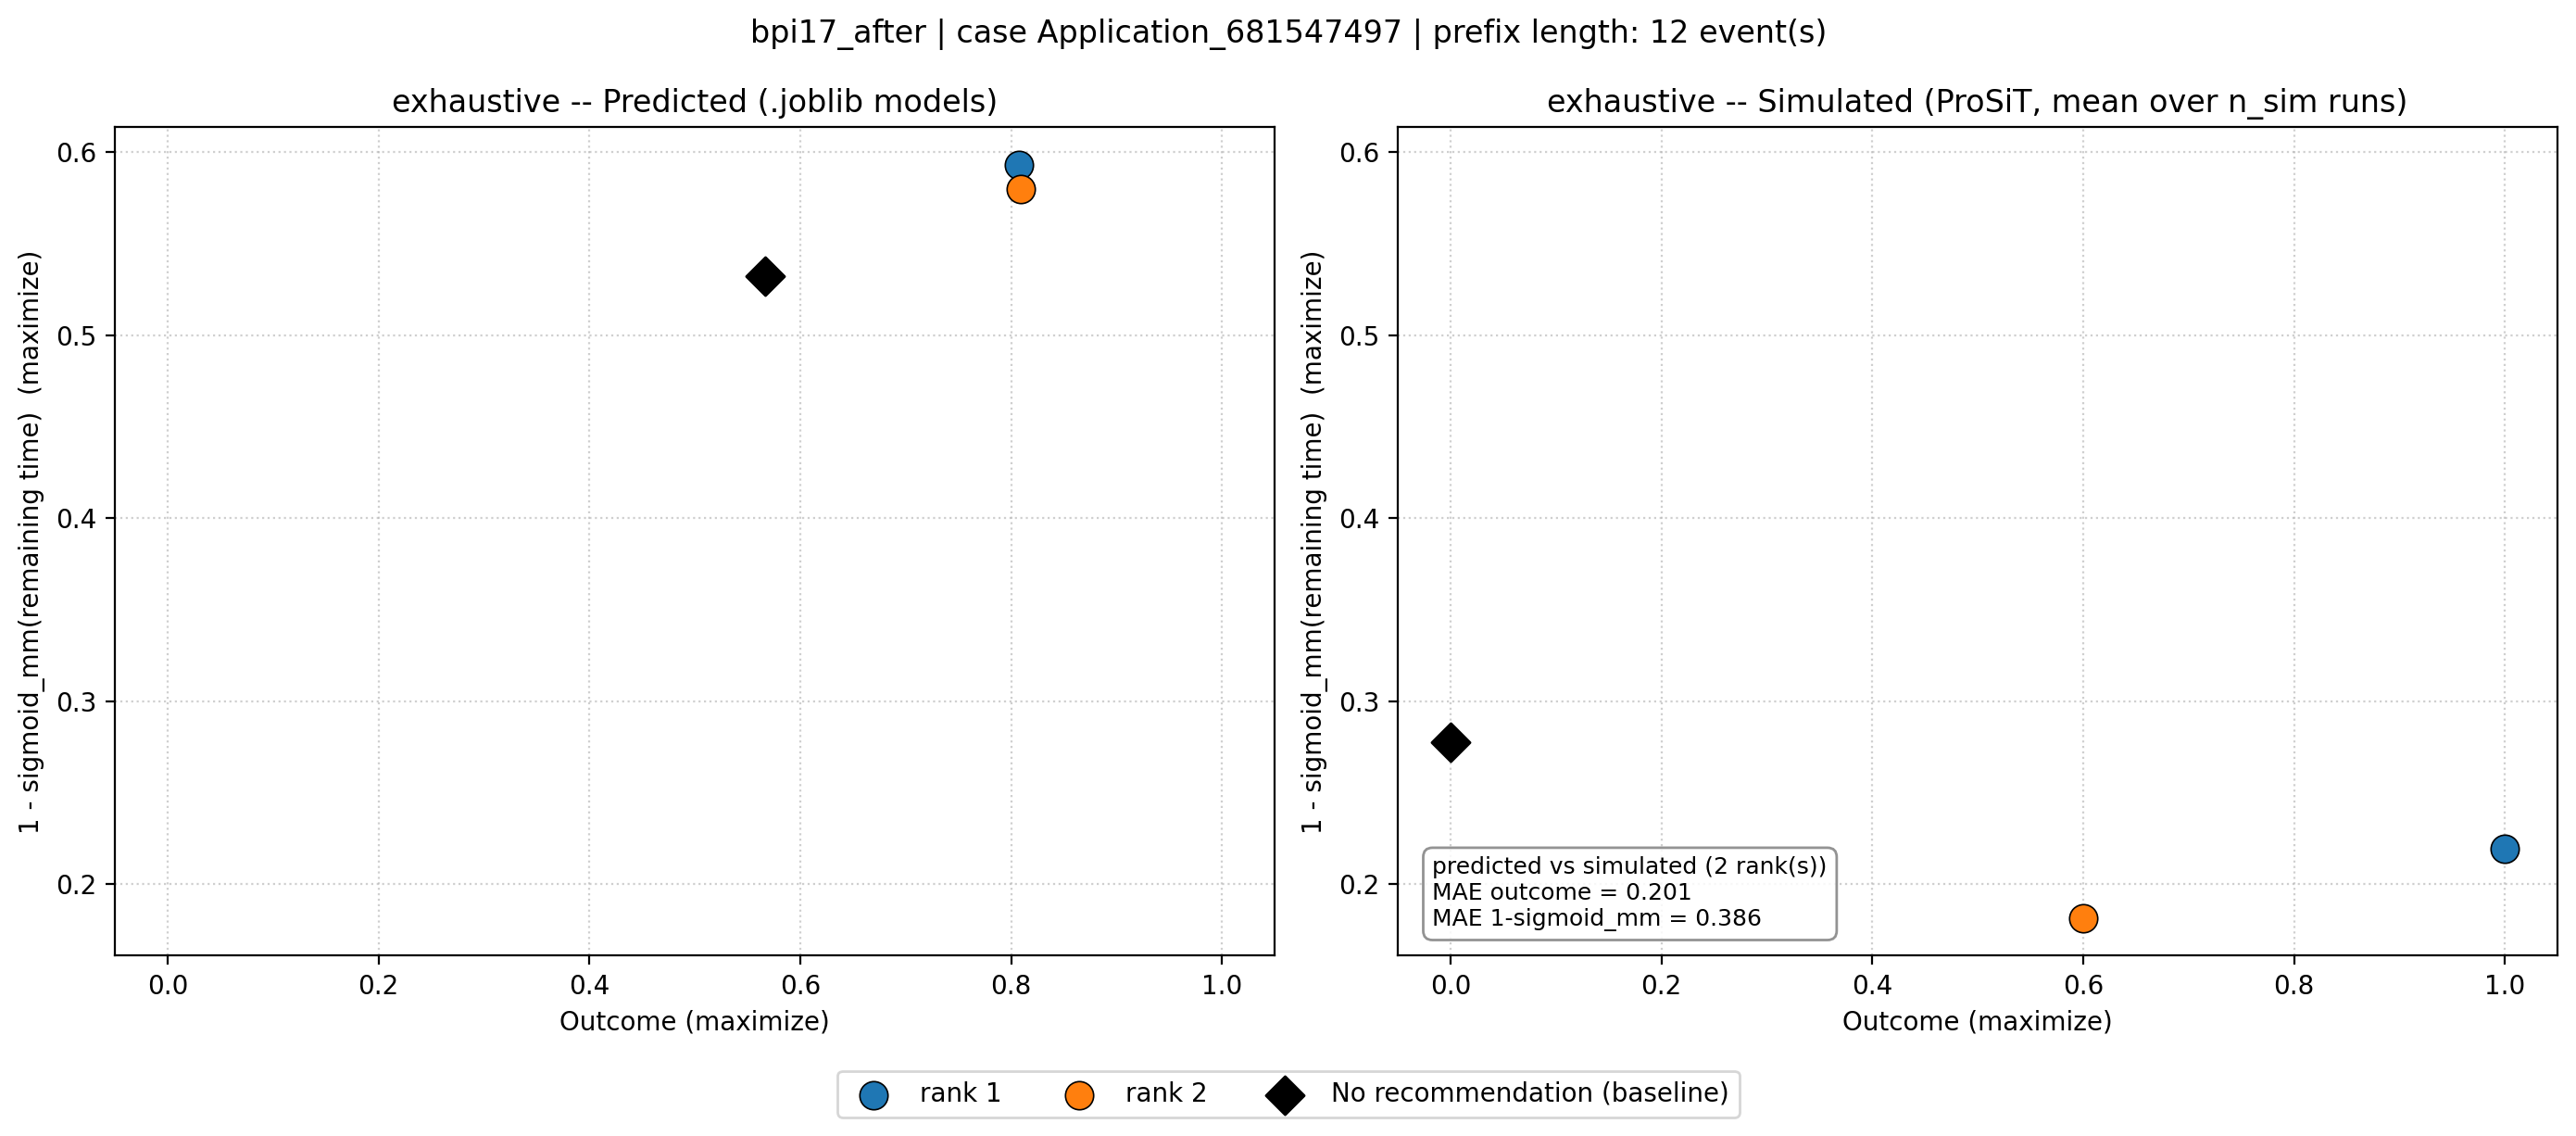
\includegraphics[width=\linewidth]{predicted_vs_simulated/bpi17_after_plots/bpi17_after_Application_681547497_exhaustive_predicted_vs_simulated.png}
    \end{minipage}
\end{frame}

\section{Threats to Validity}

\begin{frame}[plain,c]
    \centering
    \color{Darkcandyapplered}
    \Huge\textbf{Threats to Validity}
\end{frame}

\begin{frame}{Simulator Validation: Positive-Outcome Rate}
  \small
  The \textbf{baseline} simulation (test prefixes, no recommendation, 10 runs) is
  compared with two real references: the \textbf{whole log} and the \textbf{same test
  cases} it continues.
  \begin{center}
  \begin{tabular}{lccccc}
    \toprule
     & \multicolumn{3}{c}{\% positive} & \multicolumn{2}{c}{$\Delta$ baseline (pp)} \\
    \cmidrule(lr){2-4}\cmidrule(lr){5-6}
    Case study & Whole log & Test cases & Baseline sim. & vs.\ log & vs.\ test \\
    \midrule
    BAC          & 84.3 & 78.1 & 77.2 & $-7.0$  & $-0.9$ \\
    BPI12        & 47.9 & 38.7 & 44.2 & $-3.7$  & $+5.5$ \\
    bpi17-before & 56.4 & 42.0 & 39.7 & $-16.8$ & $-2.3$ \\
    bpi17-after  & 54.7 & 47.9 & 44.8 & $-9.9$  & $-3.1$ \\
    \bottomrule
  \end{tabular}
  \end{center}
  \footnotesize
  \begin{itemize}
    \item The test cases are the ones \alert{still running at the split}: they are
      less often positive than the average case of the log ($-6$ to $-15$ pp).
    \item Against the whole log the baseline seems far off (up to $-16.8$ pp), but
      most of that gap is this selection effect: against the \alert{same test
      cases} it stays within $\pm 3.1$ pp, except BPI12 ($+5.5$ pp, the simulator
      over-predicts acceptance).
  \end{itemize}
\end{frame}

\begin{frame}{Simulator Validation: Trace Duration}
  \small
  Duration of the complete traces in days, median (mean).
  \begin{center}
  \begin{tabular}{lcccc}
    \toprule
    Case study & Whole log & Test cases & Baseline sim. & $\Delta$ median vs.\ test \\
    \midrule
    BAC          & 7.7 (15.5)  & 10.5 (20.9) & 11.1 (22.6) & $+0.5$ d \\
    BPI12        & 15.1 (18.6) & 22.9 (24.4) & 29.6 (30.2) & $+6.7$ d \\
    bpi17-before & 16.1 (20.2) & 30.8 (29.0) & 30.8 (29.7) & $0.0$ d \\
    bpi17-after  & 19.9 (21.9) & 30.8 (28.4) & 30.9 (30.1) & $+0.1$ d \\
    \bottomrule
  \end{tabular}
  \end{center}
  \footnotesize
  \begin{itemize}
    \item Same selection effect: the cases running at the split are \alert{longer}
      than the average case (median $+3$ to $+15$ d), so the whole log is not the
      right reference for the baseline.
    \item Against the same test cases the median duration matches within one day,
      except \alert{BPI12}, where the simulated continuations are about one week
      too long.
    \item BPI12 fully simulated log (3748 traces generated from the arrival process,
      no real prefix): 49.9\% positive, median 18.2 d (mean 21.3), close to the
      whole log (47.9\%, 15.1 d).
    \item Absolute $\Delta$ values of the simulation-based evaluation, especially on
      BPI12, should be read with this residual gap in mind.
  \end{itemize}
\end{frame}



\end{document}
